\documentclass[10pt,oneside,fleqn,a4paper]{book}
\usepackage{eimthesis}
\usepackage{graphicx}
\pagestyle{plain}

\begin{document}
\pagenumbering{roman}

\title{Layered Animation from Captured Data}
\author{Raymond James Smith}
\centre{Centre for Vision, Speech and Signal Processing}

\renewcommand{\month}{9}
\renewcommand{\year}{1999}

\summary{This report details work undertaken during my first year of research in the CVSSP. A layered animation system is described, which allows interactive animation of scanned models as well as off-line detailed model animation. The application of this work to the creation of seamless H-Anim models is described. Plans for future work towards my PhD thesis are also discussed.}
\keywords{3D model capture, Layered animation, Deformable character animation, H-Anim}
\email{R.Smith@ee.surrey.ac.uk}
\acknowledgements{Supported by EPSRC Grant GR/89518 `Building Realistic Models for Virtual Reality and Animation'. I would like to thank Adrian Hilton and Wei Sun for their collaboration on the layered animation model during this first year, and for helping me to understand the field in which we are working.}

\makefront

\tableofcontents

\listoffigures

%%%%%%%%%%%%%%%%%%%%%%%%%%%%%%%%%%%%%%%%%%%%%%%%%%%%%%%%%%%%%%%%%%%%%%%%%%%%%%%%%%%%%%%%%%%%%%%%%%%%%%%%%%%%%%%%%%%%
\chapter{\label{ch:intro}Introduction}
\pagenumbering{arabic}
\pagestyle{headings}
This report details my work, undertaken during the first year of my research in the CVSSP, working on the project 'Functional Models: Building Realistic Object Representations for Virtual Reality and Animation' with Adrian Hilton, Wei Sun and John Illingworth. The project is concerned with the process of building models that are suitable for animation directly from scanned data, with as little manual intervention as possible. As well as making the creation process simpler, the removal of manual intervention should be able to speed up the process considerably, at least by eliminating the need for a human operator.

Model creation for animation is currently a laborious process, with most of the work being done by a skilled human operator. There is currently very little automation present in this process. In chapter \ref{ch:review}, we discuss the current state of the art in the field of 3D modeling and animation, with reference to current capture hardware, model-building processes, commercial software and character animation techniques. It is important to understand all of these field before designing a process that intends to bridge the gaps across many of them.

We are currently investigating methods for creating so-called {\it layered} models for animation directly from scanned data. The models have three layers, a skeleton, a simple control mesh, and a dense detail layer. We have developed a method for layered model construction and animation, which is discussed in chapter \ref{ch:animationchain}. The layered animation process involves capture of data, automatic model building, and animation. The bulk of my contribution to the process so far has been on the animation of these layered models, specifically of the control mesh layer, and it's application to the creation of seamless VRML humanoid models (covered in chapter \ref{ch:vrmlhumans}). Some results of this work are presented in chapter \ref{ch:results}.

Future work on the animation chain will involve increasing the level of automation in the capture and modeling process, and investigating more complex methods for animating these models at various levels of detail. In particular, the possibility of representing multiple levels of detail as a displacement map will be investigated. The goal is to achieve efficient and realistic animation, transmission and storage of layered models for Internet based applications. A discussion of plans for my future work on the project is contained in chapter \ref{ch:future}.

%%%%%%%%%%%%%%%%%%%%%%%%%%%%%%%%%%%%%%%%%%%%%%%%%%%%%%%%%%%%%%%%%%%%%%%%%%%%%%%%%%%%%%%%%%%%%%%%%%%%%%%%%%%%%%%%%%%%
\chapter{\label{ch:review}The State of the Art}

In order to develop new methods for the model creation process, we must first understand the efforts that have already taken place in the field. We must understand the scanning and modeling process, and also how the models will be animated once we have created them. Therefore, this section will review current methods for model creation and animation. This is an area with a large commercial interest, so we must understand not only academic research into these fields, but also currently-available commercial hardware and software systems. This review does not aim to be exhaustive, due to the large range of material covered, but instead to highlight major approaches in order to provide an overview of each field.

\section{\label{sec:reviewscanning}3D Scanning and Modeling}
Our layered animation chain, as with all model creation, must begin with the creation of the original model that we want to represent. This can be done by modeling an object on a computer from scratch, or it can begin with an object in the real world that we want to represent. This is the approach that we will consider, and so in order to use a real-world object in computer animation, we need to create a computer model of it. The first section of this review will concentrate on the process of capturing data about an object from the real world, and then discuss how to represent it inside the computer.

There are two main stages to the process of capturing 3D models from real objects. These are the capture process itself, in which an object from the real world is digitised, followed by a reconstruction process, in which this digitised data is rebuilt into a 3D model. However, there is also a third topic for discussion in this area, which is the method used to represent the model once it has been rebuilt.

\subsection{\label{sec:reviewcapture}3D Capture Systems}
The first stage in any 3D scanning system is the capture of data from the real world, the scanning or sensing phase \cite{Isdale98}. This involves using some kind of hardware to digitise data about the object being scanned. There are three main categories of 3D scanner. These are Tracking Systems, Imaging Systems and Range Finders. There are also systems that use a combination of these methods.

\subsubsection{Tracking}
Tracking systems capture data by positioning a probe of some kind on the object being scanned and capturing a single point at a time. Systems include Coordinate Measuring Machines (CMMs), which are generally probes attached to a mechanical arm. The arm contains sensors that measure the position of the probe when a point is captured. Other systems use different methods of tracking to provide greater freedom, such as electromagnetic and ultrasonic trackers. These can be used to capture larger objects, as the tracker is free to move over a much larger area. Systems can also be automatic or manual. Manual systems can be extremely time-consuming, as each point in the final model needs to be captured individually, but it can eliminate the need for reconstruction of the 3D model, as the points can be scanned at known positions corresponding to the desired vertices in the final model. Automatic systems produce clouds of points that need to be rebuilt into a meaningful model by a reconstruction process.

\subsubsection{Imaging}
Imaging systems use a number of 2D images which are combined to give 3D geometry data. Imaging systems work at various levels of abstraction, from systems that generate point clouds by calculating range measurements, to systems that generate a model directly by extracting feature points from the image data. Other systems use silhouettes of the object at different angles to create a volumetric model that can then be converted into a polygonal representation. Medical scanners also come under the heading of imaging systems, as they take a series of slices (which can be considered to be images) through the object to be scanned, using sensors such as MRI, CT and so on.

\subsubsection{Range Finding}
Range finding systems generally produce a 2D array of distance measurements known as a {\it range image}, which can be considered as a point cloud and reconstructed in the same way as other styles of capture. Range finding systems are mostly optical systems, using laser and white light to measure distance, although at least one ultrasonic time-of-flight based range finding system has been developed for scanning very large structures. Laser scanners work by projecting a laser stripe onto the surface being scanned, and viewing the stripe through a camera positioned at an angle to the scanner. The shape of the stripe in the camera's view can be converted into a distance measurement, in a process known as {\it optical triangulation}. Some systems are also capable of capturing texture information from objects, which can then be mapped onto the generated models. Some scanners, such as those from Cyberware move the scanner around the object automatically, but this requires a large working area and complex machinery. Quite a popular alternative technique is the combination of a tracking system and a range finder. Systems of this kind include 3D Scanner's ModelMaker, which is a CMM arm with a laser scanner on the end, and the Polhemus HLS, which uses Polhemus' magnetic tracking system and a laser scanner. This kind of system allows the scanner to be moved freely around an object, while also getting accurate position and orientation information for the scanner itself, easing the data fusion process.

\subsection{\label{sec:reviewreconstruction}3D Reconstruction}
Once the object that we want to represent has been captured, using the methods outlined above, we need to build a 3D model from the data that we now have at our disposal. In many cases, this will be in the form of a set of range images, so this is the situation we will concentrate on in this review. There are many other methods that are used to fuse data from other sensor types, such as silhouette-based systems for creating models from image data, but these will not be covered here. 

There are two main problems involved in merging multiple range images \cite{Illingworth98}. The first is the problem of {\it registration}, which involves positioning the range images correctly, relative to each other. When multiple range images are taken without information on the sensor position for each one, this is a major problem. The combination tracker/scanner systems avoid this problem, however, as the scanner position is always known. Then, we only have to solve the second problem, how to fuse the multiple range images together into a single surface, either polygonal, spline-based, or some other type that can be converted into a more widely-used surface type.

\subsubsection{Registration}
The most widely used method of surface registration is the iterated closest point algorithm \cite{Besl92}. This matches two surfaces by matching a number of points on the first surface to their closest point on the second surface. It then calculates the transformation required to align the matched points. This transformation is applied and the process repeated until the alignment does not change. This only works for surfaces that are already roughly aligned. The problem of automatically registering non-aligned surfaces is still open.

\subsubsection{Surface Reconstruction}
Once the range images are registered, we need to fuse them together into a single surface. Early approaches to this problem concentrated on fitting parametric surfaces such as deformed planes and spheres to the data. These methods have their obvious limitations, being confined to simple surfaces.

One of the early attempts at a solution using triangulated meshes was that of Turk and Levoy \cite{Turk94}. They suggested a method that used triangulated range images (essentially a number of separate meshes) and stitched or `zippered' them together. Their method involves three stages: first, the overlapping portions of the meshes are removed, so that no whole triangles from one mesh overlap the other mesh. This leaves overlaps only at the boundary of the two meshes. Then, one mesh is `clipped' against the other, producing an edge on the clipped mesh that follows the edge of the clipping mesh. All points where the two meshes intersect this new edge are made into vertices, and the meshes adjusted to include them. This is followed by calculating what is called the {\it consensus geometry}, which means that all measured points are used in an averaging of the surface. However, this approach gives a large number of small and thin triangles along the edges, and has been shown through testing to be error prone.

Rutishauser et al.\cite{Rutishauser94} describe a method for merging two triangulated range images at a time. A mutual approximation of the two is performed using an explicit error function which `fades' between the two surfaces, depending on how reliable the measurements are at the point under consideration. Then, a re-triangulation is performed to merge the two meshes into one. A feature of this algorithm that the authors point out is that the output data is in the same format as the input (i.e. a triangle mesh), so more range images can be incrementally added using the same algorithm. However, the algorithm can break down in areas of high surface curvature.

A method to create surfaces from unorganised point sets was proposed by Hoppe et al.\cite{Hoppe92}, using an implicit surface-based approach. An implicit surface is a surface that is defined not as explicit points, but as the solution to a mathematical function $f(x)=0$. This algorithm estimates an oriented tangent plane for each point, which serves as a local linear approximation to the surface. These are estimated by calculating a plane based on the points in the neighbourhood of the current point, and propagating plane orientations using the minimal spanning tree of a Reimannian Graph. The resulting tangent planes are not suitable for defining a surface, as the combination of them all may have an extremely complicated structure, so they are used to calculate a signed distance function, which is used as the function $f(x)$ for evaluation of the implicit surface. As the tangent plane for a point does not necessarily pass through that point, the assumption that the tangent planes are local approximations can be used to provide an estimate of the distance to the real surface for each point. As the planes are oriented, the distance is also signed, so a point can be said to lie either inside or outside the surface. The signed distance function defines an implicit surface, which is defined as those points $p_i=(x_i,y_i,z_i)$ such that $f(p_i)=0$ \cite{Ning93}. The implicit surface is an {\it isosurface} for the value of the signed distance function $f(p_i)=0$. This isosurface is then converted into a polygonal representation using the Marching Cubes algorithm \cite{Lorensen87}. This method works well for simple objects, but the graph calculations can be very expensive for models with a large number of points.

A number of other methods have been proposed which use the implicit surface approach used in Hoppe's work, but which build the implicit surface in different ways, using the underlying structure of the input data to improve the results.  Curless and Levoy \cite{Curless96} describe a volumetric method for merging range images. This approach converts the range image into a triangulated mesh in the same way as Rutishauser, and stores the surface in a volumetric model, a discrete 3D grid made up of semidisjoint cells called {\it voxels}. The surface is encoded implicitly in the volumetric model by calculating the signed distance from the triangulated mesh for each voxel in the volume. As new range images are added, the complete surface is built up as an isosurface inside the volumetric model. This is then polygonised using Marching Cubes. Hilton et al.\cite{Hilton96b} suggest a more robust approach, which only calculates the value of the signed distance function at precise positions as required by the Marching Cubes algorithm as it executes. This means that the signed distance function is no longer discrete, as in the voxel grid, but continuous, allowing more efficient and reliable reconstruction of the isosurface, even in areas of high curvature and thin sections. Execution is also faster as no unnecessary calculations are performed.

\subsubsection{Implicit Surface Tiling}
Once we have created an implicit surface, we need to represent it in some way that can be used for a higher-level application \cite{Bloomenthal97}. Usually the best way to do this is to convert the surface into a polygonal mesh. Fitting other types of surface is possible, but much more work has been done on polygonisation, so we will concentrate on this approach here. Polygonising, or tiling an implicit surface is the process of converting the isosurface (normally $f(p_i)=0$) into a set of polygons (usually triangles). Many approaches have been suggested for this, but we will concentrate on the most popular approach, such as is used in the Marching Cubes algorithm by Lorensen and Cline \cite{Lorensen87}.

The first stage in tiling an implicit surface is to split the volume occupied by the model into discrete semidisjoint cells, a {\it spatial partitioning}. These cells are normally cubes, as the cube is the only regular polyhedron that can fill a space without gaps or overlaps. It can also be easily subdivided into smaller cubes. One other polyhedron can do this, the{\it Kuhn simplex}, and this is used in some partitioning methods, but we will not cover it here. The value of the implicit function can be evaluated at the cell corners, giving an indication as to whether a cell is {\it transverse} (i.e. crosses the surface) or not. Transverse cells have a number of vertices with a negative value and a number with a positive value, as this indicates that the surface lies within the cell.

Early methods of polygonisation approximated the surface using the transverse faces of the cells. This gives a very blocky model, and better results are obtained by using {\it cell polygonisation}. This involves converting the transverse cells into a set of polygons, depending on the arrangement of positive and negative vertices. If an edge has a positive vertex at one end and a negative vertex at the other, the surface must cross that edge. It is at this point that the difference between discrete and continuous implicit surfaces becomes important. Discrete surfaces can only be accurately sampled at the vertices, and linear interpolation must be used to determine the crossing point on an edge. This is less accurate than a continuous approach, which can sample at any point (at higher computation cost), and so can find the exact crossing point, possibly by using some binary search approach. Once all the crossing points are found, a set of triangles can be constructed inside a cell, which correspond to the shape of the surface inside that cell (see figure \ref{fig:polygonisation}). Adjacent cells will have the same crossing points at their boundaries, so the shape of the surface will be consistent across any adjacent cells. However, for a cube, some arrangements of positive and negative vertices are ambiguous, and can be polygonised in different ways. This can cause inconsistencies in the surface, and so a consistent method of ambiguity solving is required. This can be achieved by taking more sample points within a volume, either by sampling in the centre of the cell, or by subdividing the cell into unambiguous volumes, such as tetrahedra.

\begin{figure}
\begin{center}
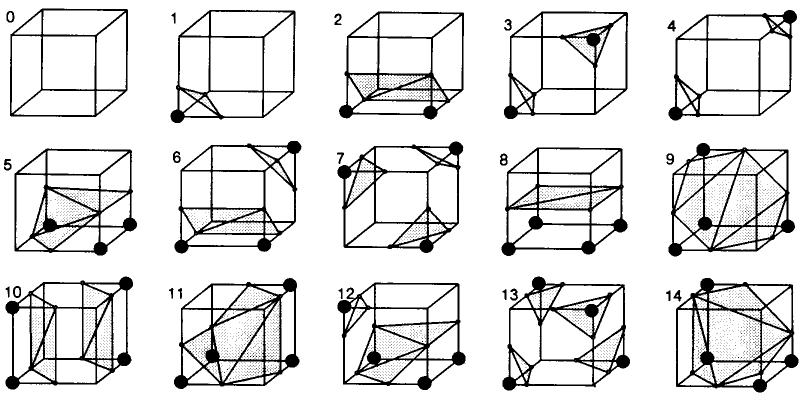
\includegraphics[height=5cm]{../images/marchingcubes}
\caption[Cell Polygonisation]{\label{fig:polygonisation} Cell Polygonisation. A transverse cell has positive and negative vertices. Surface crossing points can be found on edges that have both, and define the surface shape within the cell. Figure taken from \cite{Lorensen87}}
\end{center}
\end{figure}

Standard spatial partitioning methods of surface tiling have a number of drawbacks, including the fact that the resulting triangulation is extremely irregular. An example of an alternative approach to surface tiling that does not use a spatial partitioning is Marching Triangles, proposed by Hilton et al. \cite{Hilton96a}. This method grows a polygonal mesh across the implicit surface by using a {\it predictor-corrector} approach. Starting with a seed mesh (only one triangle is needed), for each boundary edge a new vertex position is estimated by projecting a constant distance perpendicular to the edge, in the plane of the attached triangle. This vertex position is then corrected by finding the closest point on the implicit surface, and updating the vertex position to this new point. Tests are also performed to ensure correct orientation of the surfaces, to stop the mesh growing at a surface boundary, and to stop the mesh growing over itself. This approach gives a much more efficient polygonisation, and can also cope with open surfaces. The method can also be extended to give adaptive triangle sizes by changing the projection distance.

\subsection{\label{sec:reviewsurfaces}Surface Representations}

Once a model has been digitised, we need to decide which form of surface is best suited to our needs. Up until now, we have only discussed polygonal representation of surfaces, but other representations are possible. Polygonal representations are the dominant form of surface in computer graphics. However, with the desire for realistic models, the limitations of polygonal models have become clear. Polygonal models can represent surfaces of arbitrary complexity, but have the problem that they are piecewise linear, and are therefore inefficient for smooth surfaces \cite{Besl94}. A smooth surface cannot be represented efficiently, as a close approximation would require an enormous number of polygons. This has meant that both for animation and engineering applications, smooth surfaces have received a lot of attention. In this section, we will briefly review the major types of smooth surface.

\subsubsection{Spline Surfaces}

Most smooth curves are based on the use of parametric polynomial curves, normally using a cubic polynomial as a function applied to the parameter $u$, which varies between 0 and 1 along the curve. The coefficients of the polynomial are given by a set of 3D {\it control points}, three for a quadratic curve, four for a cubic. The simplest form of smooth curve is an interpolating curve, where the curve intersects all four of the control points. Another form is the Hermite curve, where the four coefficients are two control points (one for each end) and the derivative of the curve at each endpoint. This allows the gradient at each end to be specified. The Bezier curve is a cubic polynomial that uses four control points as coefficients in the same way as the interpolating curve, but which approximates the Hermite curve. This is a simpler and more efficient method than using Hermite curves, but gives similar control over the gradients at the endpoints. B-Splines use four control points, but only define the curve between the middle two. Using B-Splines, a curve with an arbitrary number of control points can be specified, by stitching together B-Spline curve segments. If the control points for one spline overlap the control points for the next, the two will be continuous, both in their geometric positions and in their derivatives.

Smooth surface patches are an extension of smooth curves to three dimensions. Instead of a single parameter, there are two, $u$ and $v$. A smooth surface patch can be considered as the limit of the process of calculating the curve as $v$ varies for a constant $u$, or vice versa. All of the curves representations mentioned above can be extended to smooth patches. A bicubic polynomial patch (a patch that is cubic in both $u$ and $v$) will have 16 control points.

NURBS, or Non-Uniform Rational B-Splines, are a general form of B-Spline, and are now a standard curve and surface representation, as most modeling and rendering packages support the IGES file format, which is a standard format for NURBS curves and surfaces. They are particularly popular in computer graphics because they have a couple of very useful properties over normal B-Splines. First of all, normal B-Splines can be subjected to affine transformations with no problems. However, perspective transforms, such as those used in rendering, are not affine, so normal splines are not handled correctly in perspective viewing. NURBS, however, do not suffer from this, and appear as intended even after non-affine transformation. Also, quadric surfaces such as spheres, which are very useful in rendering packages, can only be approximated by nonrational B-Splines, but can be shown to be a special case of NURBS. These two properties make NURBS a very desirable choice for smooth surface representation in computer graphics. However, NURBS can only represent quadrilateral patches (a limitation of all spline surfaces), so to model a complex object will require a number of patches. These patches must also be held together, or {\it stitched}, so that gaps do not appear during animation.

Forsey and Bartels \cite{Forsey88} describe another extension to B-Spline surfaces, the {\it Hierarchical B-Spline patch}. These patches can be refined as required (for instance in areas of high surface detail) by adding extra control points between the original ones, providing a higher-order surface in the immediate area. This means that areas of a model with low surface detail can be represented with a low number of control points, whereas areas with a large amount of detail, and hence a higher order, can be represented with a more detailed surface representation.

\subsubsection{Subdivision Surfaces}
Another form of smooth surface representation is the {\it subdivision surface}. These types of surfaces have gained considerable popularity recently, and are incorporated into a number of rendering packages. A subdivision surface is a smooth surface defined, again, by a set of control points. This time, however, the control points can define an arbitrary mesh, not just a quadrilateral patch with a particular number of control points. The edges and faces of the control mesh are subdivided or refined by some algorithm. The subdivision surface is defined as the limit of the refinement process applied to the control mesh. There are three main types of subdivision surfaces, each with their own subdivision algorithm and style of control mesh. The three types are Doo-Sabin \cite{Doo78}, Catmull-Clark \cite{Catmull78}, and Loop \cite{Loop94} surfaces. Doo-Sabin surfaces are based on the subdivision of quadratic uniform B-Spline surfaces, and subdivide by dividing each vertex into {\it n}, where {\it n} is the number of faces adjacent to the vertex. The new vertices are the average of the original vertex, the centroid of the face, and the midpoints of the two edges adjacent to the face and the original vertex (see figure \ref{fig:subdivision}a). Catmull-Clark surfaces are based on the subdivision of cubic uniform B-Spline surfaces, and create a number of different kinds of new vertices at each subdivision step. New {\it face points} are the average of all the old points defining a face, new {\it edge points} are the average of the midpoint of an old edge with the average of the two new face points of the faces sharing the edge, and new {\it vertex points} take into consideration adjacent face points, midpoints of adjacent edges, and the original vertex (see figure \ref{fig:subdivision}b). Both of these schemes work on control meshes of arbitrary topology, as opposed to Loop subdivision, which uses control meshes composed only of triangles. Loop subdivision , which is based on the subdivision of quartic uniform box splines, divides each triangular face into four smaller triangular faces, while moving the vertices (see figure \ref{fig:subdivision}c). Subdivision surfaces can be extended to allow sharp edges by constraining the subdivision routine. Hoppe \cite{Hoppe94a} did this for Loop surfaces, and DeRose et al.\cite{DeRose98} have developed a similar method for Catmull-Clark surfaces.

\begin{figure}
\begin{center}
\begin{tabular}{ccc}
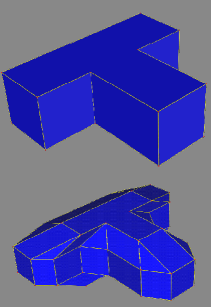
\includegraphics[height=6cm]{../images/doo-sabin} &
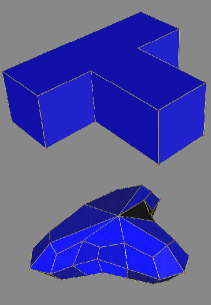
\includegraphics[height=6cm]{../images/catmull-clark} &
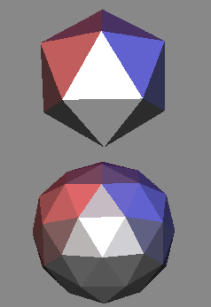
\includegraphics[height=6cm]{../images/loop} \\
{\it(a)} & {\it(b)} & {\it(c)}
\end{tabular}
\caption[Subdivision Surfaces]{\label{fig:subdivision} Subdivision Surfaces. (a) Doo-Sabin subdivision. (b) Catmull-Clark subdivision. (c) Loop subdivision.}
\end{center}
\end{figure}

\subsection{\label{sec:reviewdetail}Representation of Surface Detail}

A polygonal or smooth surface can represent the gross shape of an object efficiently, but real objects have surface detail, such as wrinkles in skin and so on. These are difficult to represent unless the model is extremely detailed. A polygonal model would require a very large number of faces to represent small surface details, and a smooth surface would need a large number of patches or control points. Large numbers of polygons or control points will increase rendering time, and therefore prohibits interactive animation. Therefore, a number of tricks have been developed that can be used to fool the viewer of a model into thinking that there is more detail in the surface than is actually present.

The simplest of these is {\it texture mapping}, where an image of the surface of the real object is mapped onto the surface of the model. This can give the appearance of surface detail that is not really present, but has the problem that it will not change with lighting. Also, the surface is still obviously the simple shape when examined closely.

Another approach is {\it bump mapping}, proposed by Blinn \cite{Blinn78}, and is used during shading of the surface. A bump map is a texture used to perturb the normals of the surface during shading. This changes the lighting on the surface, making it appear as if the surface detail is present. The actual surface is still the original shape, but this is only obvious if the viewer looks across the surface, where no change in the surface can be seen.

The last alternative we will cover is {\it displacement mapping}, which actually perturbs the shape of the surface \cite{Cook84}. A displacement map consists of a series of offsets which are mapped onto the surface. During rendering, a new surface is created which includes all of the surface detail from the displacement map. As this approach actually moves the surface, the result is indistinguishable from a very dense mesh. Adaptive level of detail is possible with all of these approaches,  depending on how closely the viewer is looking at the object.

\subsection{\label{sec:reviewmodeling}Modeling Techniques}

There is no standard method for creating digital models for animation, especially from scanned data. Many models are created purely in software tools, with no reference to real life objects, but this does not fit well into a typical animation house, which is used to skilled artists creating real models. For this reason, many use clay or other materials to create a model that can then be digitised. However, approaches to reconstructing a model from scanned data differ widely. The problem is that dense polygonal models (the dominant form of output from scanning software) are inappropriate for use in animation. The models have far too many faces to be usable in an animation package, and the mesh is normally completely unstructured. This is no good for animation, where the model needs to be structured so that the surface can move sensibly when the model is animated.

Most computer-generated characters are designed manually on a computer, with no reference to the real world. Alternatively, a real model can be digitised by using a touch probe (CMM). particular points on the surface of the model are measured, and the mesh reconstructed directly from the scanned points. This allows rapid construction of a 3D model, but the mesh must be effectively designed by hand before scanning. This is the approach taken by Viewpoint Datalabs, a well-known supplier of 3D models for animation.

Another possibility is that a model will be scanned and reconstructed into a dense point cloud. The points are then joined by hand to create the polygonal representation. This allows a highly structured mesh to be constructed, but is incredibly labour-intensive and takes many days of skilled work to remodel an entire character. At present, this is the approach that is used by many animation houses, including Jim Henson's Creature Workshop.

Animation systems that require an extremely accurate look, particularly for modeling realistic objects, use a highly layered anatomical approach. A skeleton model will be built, and then a muscle layer added on top of this. The scanned skin layer will sit on top of this model, sometimes with an extra layer in between to simulate body fat. Needless to say, this approach requires a great deal of skill to model, and a great deal of processing time to render and animate. The results, however, can be highly realistic.

Another approach is to fit some kind of smooth surface model to the scanned data. Usually, this involves fitting stitched NURBS patches to the surface, but other approaches have been used. Recently, Pixar have had some success in modeling surfaces using Catmull-Clark subdivision surfaces \cite{DeRose98}. For their short film {\it Geri's game}, they created the head, hands and clothing of the main character using these surfaces. They used a process whereby a clay model of the head was sculpted, and then points on this model digitised using a CMM system. These scanned points were then used as control points for the subdivision surface, illustrated in figure {\ref{fig:geri}}. Also, the Catmull-Clark subdivision method was extended to allow sharp creases, in a similar way to Hoppe's work on Loop surfaces. The use of subdivision surfaces allows the creation of completely seamless smooth surface models, as opposed to more standard methods using NURBS, where different patches of the same surface must be held together explicitly. Geri looks very good, but he is not a realistic character, so the more realistic layered methods are not required.

\begin{figure}
\begin{center}
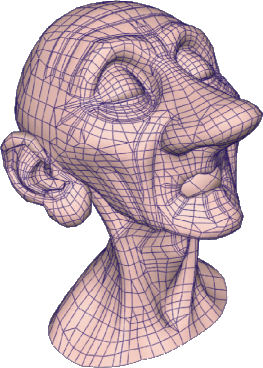
\includegraphics[height=5cm]{../images/geri_control}
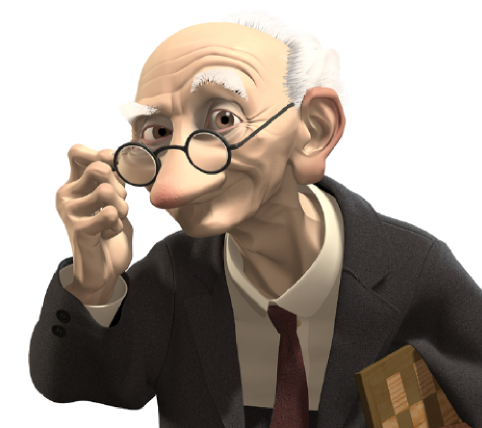
\includegraphics[height=5cm]{../images/geri2}
\caption[Pixar's Geri]{\label{fig:geri}Pixar's Geri, from their short film {\it Geri's game}. A clay model of the head is digitised at particular points to obtain control points for a Catmull-Clark subdivision surface. Images taken from \cite{DeRose98}.}
\end{center}
\end{figure}

Krishnamurthy and Levoy \cite{Krishnamurthy96} describe a method which uses both the polygonal and smooth surface approaches. A model is scanned and converted into a dense polygon mesh. This is then split into sections manually by drawing curves on the mesh, and a B-Spline patch is fitted to each section. Also, a displacement map is generated for each patch, which encodes the errors between the original surface and the B-Spline patches. The B-Spline patches therefore define the overall shape of the model, and the displacement maps provide the surface detail. However, the method does not define any method for animation of these models.

\subsection{\label{sec:reviewsoftware}Commercial Modeling Software}

There are a number of commercial software packages than incorporate some of the modeling techniques described above. Finally in this section, we will present a short overview of some of these packages in order to show the typical approaches used in commercial packages.

Remesh, from 3D Scanners ({\it http://www.3dscanners.com}), takes the approach of trying to ease the process of creating a structured polygon mesh from scan data. Normally this would require a large amount of manual work, as mentioned above, but Remesh allows the modeler to create a structured mesh from the original scan data without joining data points by hand. Once the dense mesh has been created, the modeler can draw curves (or {\it polylines}) across the surface of the mesh. These join up to create either triangles or squares of polylines, which define a patch (see figure \ref{fig:remesh}b). Once the curves have been drawn, the polylines are subdivided into $n$ sections, and the patches are divided into $n*n$ sections (see figure \ref{fig:remesh}c). The corners of these sections follow the surface of the mesh. The sections are then converted into polygons, creating a new mesh (see figure \ref{fig:remesh}d). This is basically a controlled resampling of the scan data,  with the density and positions of the sampling points controlled by the modeler. One problem of this approach is that patches must be quadrilateral or triangular, and each patch is subdivided equally. This can lead to a wide variation in the resolution of the resulting model.

\begin{figure}
\begin{center}
\begin{tabular}{cccc}
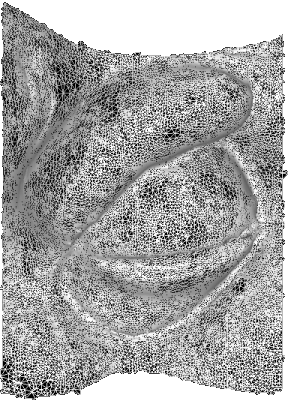
\includegraphics[width=3.18cm]{../images/eye_dense} &
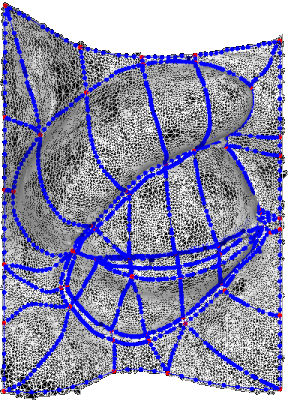
\includegraphics[width=3.18cm]{../images/eye_polylines} &
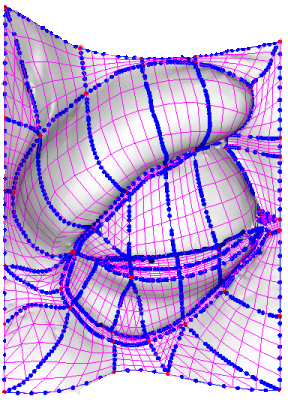
\includegraphics[width=3.18cm]{../images/eye_generate} &
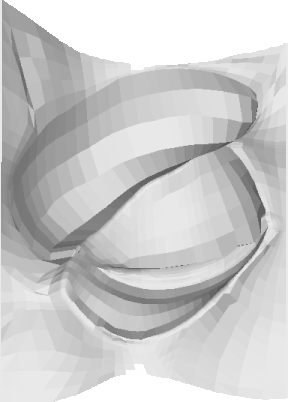
\includegraphics[width=3.18cm]{../images/eye_remesh} \\
{\it(a)} & {\it(b)} & {\it(c)} & {\it(d)}
\end{tabular}
\caption[The 3D Scanners Remesh re-modeling process]{\label{fig:remesh}The 3D Scanners Remesh re-modeling process. (a) The scan data is reconstructed into a polygonal mesh. (b) Lines are drawn onto this mesh, splitting the surface into patches. (c) The patches are subdivided equally, with the subdivisions following the surface, which then are used to create a remodeled mesh (d).}
\end{center}
\end{figure}

Paraform ({\it http://www.paraform.com}) is a package that implements the modeling approach proposed by Krishnamurthy in \cite{Krishnamurthy96}, described above. This creates a dense polygon mesh from scan data, to which smooth surface patches are fitted. This creates models that are represented as NURBS patches with surface detail maps (either bump maps or displacement maps) layered on top. These models can then be imported into many commercial animation and rendering packages. Geomagic Shape ({\it http://www.geomagic.com}) and Cyberware's CySlice ({\it http://www.cyberware.com}) also create similar models based on NURBS patches. None of these packages generate models in a form directly suited to animation. In all cases this is done in an external rendering and animation package, such as 3D Studio MAX or Maya.

\section{\label{sec:reviewcharacter}Deformable Character Animation}
One of the most important applications of model-building from scanned data, at least for the entertainment industry, is the creation of character models that can be animated. Obviously, being able to scan rigid objects is useful, but ideally, we want to be able to create models that are not rigid, and that can move and bend. In short, we should be able to easily create {\it deformable} models. Creating a deformable model is not really any different from creating a rigid model, apart from that we need to ensure that the model is correctly structured for animation. Topics such as surface structure and representation were covered in the previous section of this review. It is the job of the animator to decide upon a suitable layout and representation for his models. 

A deformable character will also have some kind of internal {\it skeleton}, which governs how the model moves. The skeleton is made up of bones (or {\it segments}), connected at joints. These are normally just lines, so that the skeleton appears to be a simple stick figure. Also, the skeleton is not an object in the same way as the model, but is simply a control structure used to move the model. The difficult part of deformable character animation comes when the skeleton structure is animated. The joints can rotate, and the skin of the model needs to move with them. In general, deformable characters will be {\it seamless}, in that they will be composed of a single surface (or set of stitched surfaces in the case of patch-based models). Simple character models can be built with separate objects for each body segment, but this does not appear realistic around joints in the model, so is not suitable for animation. In this section, we will cover some of the approaches to deformable character construction, and how these different construction types can be deformed during animation.

There are two main types of deformable character animation. The first type consists of the geometric approaches, where there are only two model layers, the skeleton and the skin. The skin is deformed with the skeleton in a purely geometric manner. The other type consists of physics-based and anatomical approaches, which try to model the body of the character in a much more accurate and realistic way, adding intermediate layers that emulate the body's structure in anatomical methods, or that provide some physics-based layer, such as simulation of springs between the skin and the skeleton. Also, some systems use elements of both geometric and physics-based methods. We will present examples of each of these approaches in turn, starting with the geometric models.

\subsection{\label{sec:reviewgeometric}Geometric Methods}
Geometric approaches to deformable character animation have the advantage that the skin layer is operated on only by a fairly simple geometric transformation, as opposed to complex physical or anatomical simulations, making them faster to calculate, and hence more appropriate for real-time applications. A number of different methods fall under the category of geometric methods. We will discuss a number of these in turn.

\subsubsection{Free-Form Deformations}
Some deformation methods that can be applied to character animation are independent of the method of construction of the underlying model. On of these is the Free-Form deformation method, described by Sederberg and Parry in \cite{Sederberg86}. FFD is a very flexible method of surface deformation. The key to the system is that it does not deform the object directly. Instead, it embed the object in a space which is then deformed. This allows FFD to work on any type of surface representation. FFDs are based on trivariate Bernstein polynomials, and can therefore be considered to be a three-dimensional extension of the deformation of a flat surface patch by moving control points. The object to be deformed is embedded in a tricubic Bezier hyperpatch, which has 64 control points. These control points can be moved, and the hyperpatch changes shape in a manner that Sederburg calls `intuitively consistent'. FFDs can be applied globally to a model, or only locally. If a FFD block is placed around part of a model, that part can be modified without affecting the rest of the model. This makes FFDs a popular tool in character animation. An FFD block can be placed around a joint and some of the control points attached to the skeleton. When the skeleton moves, the smooth nature of the Bezier hyperpatch ensures that the surface is smooth across joints.

The FFD method has been extended by Coquillart \cite{Coquillart90} to allow arbitrarily shaped FFD spaces to be created by combining a number of FFD lattices, a technique known as Extended Free-Form Deformation (EFFD). MacCracken and Joy further extend the FFD method to allow lattices of arbitrary topology \cite{MacCracken96}.

A popular technique in articulated character construction is to use partially overlapped FFD blocks around a joint. One FFD is applied, followed by another. In the area in which the two blocks overlap, points are deformed twice. The results from this process can be somewhat unpredictable, as it is difficult to control the deformation in the region in which the FFD blocks overlap. Therefore it is only useful in simple cases.

Chadwick et al. \cite{Chadwick89} present a more effective approach, known as {\it Critter}. This system represents a deformable character as three layers. The bottom layer is the articulated skeleton. Attached to this is a muscle layer, represented as a set of FFD blocks attached to the skeleton. Embedded within this is a layer, which is deformed by the FFD muscle layer. Despite having a third layer for the muscle, this is still a geometric model, as the muscle layer is a geometric procedure, not a complex physical simulation. The construction of the FFD muscle layer is important.  An FFD block is placed around each joint, and also along each segment. The planes of the FFD block are attached to points on the segments, and end planes of the FFD blocks are held together, so that if one deforms, the blocks next to it will also be affected. The control points within an FFD block are controlled by movements of the joints, depending on the type of FFD block under consideration. Flexor muscles (those positioned along segments) are scaled orthogonally to the segment to simulate muscle inflation. Control planes of tendon muscles (those around the joints) are rotated according to the rotation of the joint, and have a threshold beyond which creasing of the muscle occurs (control planes intersect each other).

\subsubsection{Joint-Dependant Local Deformations}
Joint-dependent Local Deformation (JLD) operators are proposed by Magnenat-Thalmann et al.\cite{Magnenat-Thalmann88}, specifically for hand deformations. The method uses only two structural layers, the skeleton and the skin. The skin model is mapped to the local coordinate system of the segment to which it is attached, ensuring that as the skeleton moves, the skin remains mapped around it. The JLD operators are functions unique to a particular joint, and are only applicable to a part of the surface (the {\it domain} of the operator). They define how the skin model deforms in that region, and simulate rounding of the skin layer close to the joints and muscle inflation along associated segments. This method has been integrated into a complete human simulation package, and has been used in the creation of various computer-generated films, such as `Rendez-vous in Montr\'{e}al' (1987).

\subsubsection{Hierarchical B-Spline Models}
We will now discuss a number of methods which are dependent on the construction method of the character model. Forsey describes a method of constructing articulated characters using hierarchical B-Splines in \cite{Forsey91}. Control points for the B-Splines are attached to the segments of the skeleton, so that the smooth surface follows the movements of the joints. This is enough for gross movement of the surface, but detailed movements around the joints cannot be represented in this way. Therefore, the area around the joint is split into a number of subsegments, between which the rotation angle is divided up, giving a smoother joint in the skeleton. Extra control points can then be added to these, giving extra control around joints.

\subsubsection{Metaballs}
Shen and Thalmann \cite{Shen95} describe a method of modeling shapes using metaballs and splines. Metaballs are an implicit surface model of an ellipsoid, and are widely supported in animation systems. Starting with a skeleton model, metaballs are added around the skeleton to build up the surface of the body, simulating the appearance of muscles and so on. There is not actually any precise relation between the metaballs and real muscles, however, making the modeling process completely subjective on the part of the modeler. The parameters of the metaballs, such as major and minor axes, can be made dependent on joint angles, so that the metaballs change shape as the body moves. Once the metaball body is in the required pose, it can be converted into a polygonal representation for display. At regular intervals down the segments of the skeleton, rays are cast orthogonally from the segment to the surface of the metaball body. The positions of the intersections with the surface become the vertices of the polygonal model. The model is therefore arranged in contour with a consistent number of vertices around each contour for each segment. 
This approach, though realistic, takes a lot of calculation, as the skin layer is reconstructed completely every time the body is moved. Thalmann et al. \cite{Thalmann96} propose a method whereby the polygonal surface of the model is generated once after modeling, and all deformation is done directly on the polygonal model. This is done by rotating the contours of the generated model, and is fast enough to allow real-time deformation of the body. The contours of each segment are rotated depending on the orientation of the joints at either end. This deformation method has been implemented in the first deformable characters for VRML by Babski and Thalmann \cite{Babski99}, and is described in more detail in section \ref{sec:reviewvrml}.

\subsection{\label{sec:reviewphysics}Anatomical and Physical Methods}
Physical methods of character animation usually involve some aspect of physical simulation, normally a simple spring-based model. Anatomical methods usually construct a model that has several highly realistic layers, and as such are almost always unsuitable for animation in real time. Also, usually these models are very complex to build, and require the modeler to specify weighting parameters for the amount of deformation, dependent on the muscle or skin area being modeled. This is a very difficult process, and is not suited to rapid construction of models.

\subsubsection{Layered Deformable Bodies}
Gascuel et al. \cite{Gascuel91} propose a method that uses three layers to construct a body model. The top and bottom are the skin and skeleton as usual, but the middle layer consists of a physical spring simulation. Springs are attached to the skeleton at one end, and the other end can move freely along it's main axis, which is fixed. Extensions of springs are also propagated to springs in the surrounding area, so that deformations are consistent within a small area. The free end of the spring governs the deformation of the skin layered above it, as the ends of the springs are used as control points for a B-Spline surface. This approach is simpler than a complex muscle simulation, and so can be computed in a reasonable time. Collisions between body parts are also modeled by this system, so that realistic deformations around the inside of joints are obtained.

\subsubsection{Anatomical Modeling}
A method for anatomically-based body modeling is proposed by Nedel and Thalmann in \cite{Nedel98}. Their models consist of a large number of physically accurate muscles attached to accurate points on a skeleton model. Needless to say, the modeling effort required to create this kind of model is very large. The models are, however, based in reality, so the modeling process is not as subjective as for the metaball method described above. The skeleton can be moved, and the muscles deform in a physically accurate way. The skin model is the generated after each movement in the same way as Shen's method for metaball modeling, by casting rays from the segments out to the surface of the muscles and generating contours for a polygonal model.

\subsubsection{LEMAN}
The LEMAN (Layered Elastic Model ANimation) system, developed by Turner \cite{Turner93}, combines aspects of geometric methods, physics-based methods and anatomical methods. It defines a body made from many layers, each with their own set of properties and deformation method. There are four layers, the skeleton, muscle, fat and skin layers. The skeleton layer is the normal jointed skeleton model. On top of this there is the muscle layer. This is composed of geometric surfaces, such as spheres or superquadrics. These are deformed using a simple geometric deformation method dependent on joint angles and the pose of the skeleton. The deformations of the muscle layer are used to calculate forces on the skin layer using a simplified spring model, through connective tissues (basically springs) that are attached to the muscles at one end and the skin at the other. The springs have parameters that govern how the skin moves over the muscle for different areas of the body. The fat layer is simply modeled as a constant thickness, to keep the skin away from the muscles. Finally, the skin layer is a physics-based model of an elastic surface. The movement of this surface is attached via the connective tissue to the muscles. 

\subsection{\label{sec:reviewvrml}Character Animation in VRML}
High-quality animation is not the only use for deformable characters. As the 3D Internet grows, demand will increase for high-quality representation of articulated characters in a standard format. As VRML97 \cite{VRML97} is currently the dominant format for 3D models on the Internet, we need to understand how character animation is performed in this language. The H-Anim specification \cite{HANIM99} defines a method for representing articulated humanoid characters in VRML, but due to the limitations of VRML97, it cannot currently support seamless deformable models. All H-Anim models are made from separate rigid segments, which look unrealistic around the joints, and have problems of surface and texture discontinuity. The H-Anim specification is discussed in detail in section \ref{sec:vrmlhanim}.

Little work has been done in the area of creating seamless deformable models in VRML. At the time of writing, only three systems (including our own) implement seamless deformable characters in VRML. One of these is by Lionhearth (http://www.lionhearth.com), but no information is available on this method, as they have chosen not to release a description to the community as yet. The only method that has been published is described by Babski and Thalmann in \cite{Babski99}. This system is an implementation for VRML of the contour-based deformation proposed by Thalmann et al.

Each segment of the body is defined as a set of contours (see figure \ref{fig:babskimodels}a). The last contour of one segment is also the first contour of the next, ensuring that the body appears seamless. When a joint rotates, the contours close to the end of a segment are rotated by different amount, varying from no rotation to half of the rotation of the joint (see figure \ref{fig:babskimodels}b). This contour rotation is applied on both sides of a joint, preserving the model's seamless appearance. The deformation can be executed in real time, due to the simple and efficient nature of rotating complete contours at the same time. However, the deformation method does suffer from thinning of segments due to the contour rotation, and also cannot handle segments that have more than two joints (e.g. the pelvis).

\begin{figure}
\begin{center}
\begin{tabular}{cc}
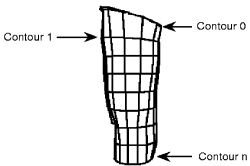
\includegraphics[height=3.5cm]{../images/babski_contours} &
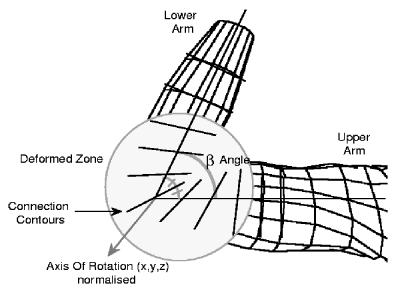
\includegraphics[height=3.5cm]{../images/babski_deformation} \\
{\it(a)} & {\it(b)}
\end{tabular}
\caption[Contoured models for VRML animation]{\label{fig:babskimodels}Contoured models for VRML animation. (a) Model structure for a single body segment. (b) Contour-based deformation around joints. Images taken from \cite{Babski99}.}
\end{center}
\end{figure}

%%%%%%%%%%%%%%%%%%%%%%%%%%%%%%%%%%%%%%%%%%%%%%%%%%%%%%%%%%%%%%%%%%%%%%%%%%%%%%%%%%%%%%%%%%%%%%%%%%%%%%%%%%%%%%%%%%%%
\chapter{\label{ch:animationchain}The Layered Animation Chain}
A fundamental difficulty in 3D computer animation is building models that are required to have not only high-detail and realistic surfaces but also believable deformations. Advances in 3D sensor technology have supplied an efficient way to capture photo-realistic 3D models of real objects. However, reconstructed surface models are usually composed of a dense, unstructured polygonal mesh representing the surface detail of the object at the resolution and accuracy of the sensor. Such meshes are notoriously expensive to store, transmit, render, and are awkward to animate \cite{Thalmann96}. The goal of this research is to enable rapid reconstruction of models suitable for animation from captured data \cite{Sun99}.

\begin{figure}
\begin{center}
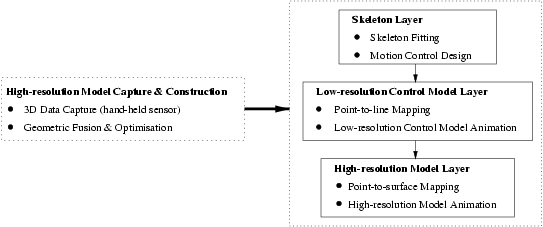
\includegraphics[height=4cm]{../images/chain_overview}
\caption[Layered Animation System]{\label{fig:chainoverview} Layered Animation System.}
\end{center}
\end{figure}

Figure \ref{fig:chainoverview} shows an overview of our system for capture and animation of 3D models. The system consists of two parts: model construction and layered animation. In the first part, a hand-held sensor system is used to capture surface measurements from 3D objects in the real world. A high-resolution triangulated surface representation is then generated using a local implicit surface based geometric fusion algorithm.

Typically,surface models  reconstructed from captured data are composed of millions of polygons and the articulation structure of the object is unknown. To animate captured models directly is expensive and it is difficult to achieve a satisfactory result. There are many different tasks such as motion control and realistic model deformation involved in animation design. In our approach, a layered model is built to enable realistic animation, in which each layer performs different animation tasks. The layered model allows an animator to manipulate a low-resolution model in real-time and render the full surface detail off line to achieve full realism.

This approach provides a relatively fast and simple technique for building animated models from captured surface measurements. The resulting model gives an efficient, realistic animation of the detailed surface while providing a low-resolution control structure for real-time interactive animation.

\section{\label{sec:chaincapture}Data Capture}
The first stage in the process is the capturing of dense surface data from the object to be modeled. This is done using a hand-held range sensor, the ModelMaker from 3D Scanners (see figure \ref{fig:modelmaker}). After the data is captured, a polygonal mesh is created, using the Remesh software package, also from 3D Scanners. The fusion and mesh generation performed by this software is based on the method proposed by Hilton et al. in \cite{Hilton96b} and described above in section \ref{sec:reviewreconstruction}. The result of this process is a very dense, high-resolution mesh of the scanned object. This will constitute the detail layer of our model.

\begin{figure}
\begin{center}
\begin{tabular}{cccc}
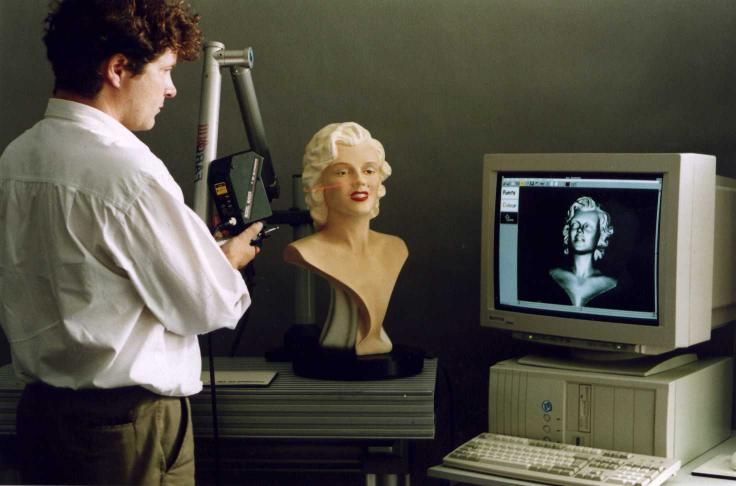
\includegraphics[height=4cm]{../images/modelmaker} &
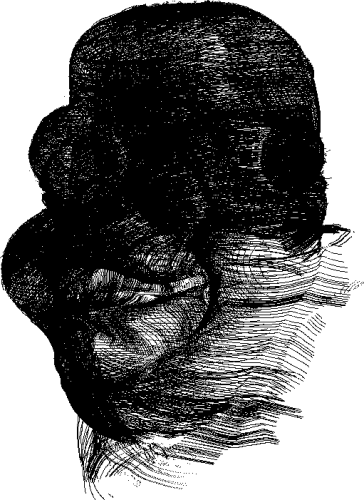
\includegraphics[height=4cm]{../images/scandata} &
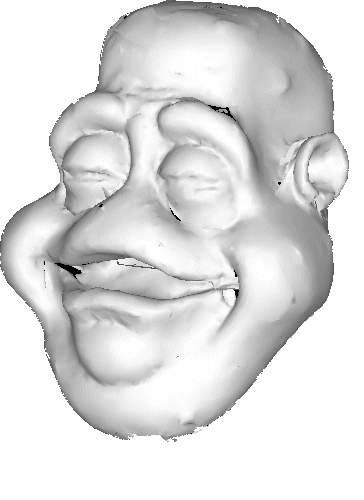
\includegraphics[height=4cm]{../images/decimated_smoothshaded} \\
{\it(a)} & {\it(b)} & {\it(c)}
\end{tabular}
\caption[3D Scanners ModelMaker]{\label{fig:modelmaker} 3D Scanners ModelMaker. (a) The ModelMaker is a laser scanner attached to a CMM arm. (b) Raw scan data points. (c) A polygonal mesh generated from the scan data.}
\end{center}
\end{figure}

\section{\label{sec:chainmodeling}Layered Model Construction}
As mentioned above, the models we will generate consist of three layers. The lowest layer in our system is a skeleton layer. A hierarchical skeleton structure is fitted interactively to the high and low resolution mesh models. The skeleton model can be animated using common animation techniques such as keyframing, inverse kinematics, physics-based models or motion capture techniques. The addition of the skeleton layer greatly simplifies the process of animating the captured model. The motion of the skeleton, which is easily defined, can provide control of all the higher layers.

The middle layer is a low-resolution control model. Although the skeleton alone is sufficient for motion control purposes, it is often too simple to be used as a representation of an object during animation design. On the other hand, the high-resolution model is prohibitively expensive to work with. Therefore it is desirable to introduce an intermediate layer. The control model is a representation of the object with the same basic shape and topology as the captured data, but a much lower polygon count. It can be a box-like model as in Kinetix's Biped for 3D Studio MAX or more complicated structured model such as those available from Viewpoint Datalabs and REM Infografica.

The top layer consists of the high-resolution captured data. This is mapped to the control mesh, to allow automatic animation of the surface detail when the control mesh is animated. The intention is to introduce this detail layer in the final rendering stage of animation to obtain a realistic model of the object.

\subsection{\label{sec:chainskeleton}Skeleton Fitting}
Using skeleton models for motion control design is a common practice for character animation. The skeleton reflects the structure of an articulated figure and is used to define the joint angles and their relationships. It enables real-time manipulation of the articulation structure to define believable animations.

The process of fitting the skeleton to the captured model requires joint positions to be identified. In our system a manual process is used to position the skeleton inside both the captured detail layer and the low-resolution control model. An interface that allows a user to identify the joint positions on a computer screen using the mouse has been developed. This is achieved by manipulating the skeleton joint positions in two orthogonal views, following the hierarchical order of the skeleton structure (i.e. fitting the root joint first and going down the hierarchy), as illustrated in Figure \ref{fig:skeletonfitting}. This allows the skeleton joint locations to be moved so that the joints are in the correct positions and the segment links between joints run through the main structures of the model. This manual skeleton positing is used as the basis for automatic mapping to form a layered animation model. The skeleton is fitted inside both the control model and the detail model to facilitate a mapping between the two.

\begin{figure}
\begin{center}
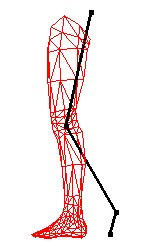
\includegraphics[height=6cm]{../images/fit1}
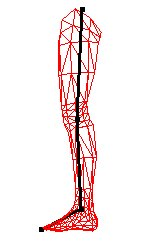
\includegraphics[height=6cm]{../images/fit2}
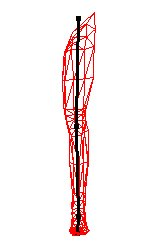
\includegraphics[height=6cm]{../images/fit3}
\caption[Manual Skeleton Fitting]{\label{fig:skeletonfitting} Manual Skeleton Fitting. The skeleton is fitted to the data in two orthogonal views.}
\end{center}
\end{figure}

\subsection{\label{sec:chaincontrol}Control Model Mapping}
Once the skeleton is fitted to the two meshes, we need to connect the layers together. We calculate a mapping of the control mesh to the skeleton, so that when the skeleton is moved, the control mesh will move with it in a consistent manner. We do this in two stages. First, we decide which segment of the skeleton a vertex in the control mesh should be mapped to, and then we parameterise the vertex in a manner local to that segment. Therefore, when the segment moves, the local coordinate system of the segment will change, and the vertices of the control mesh will move with the skeleton.

\subsubsection{Point-to-Line Mapping}
The mapping of the control mesh to the skeleton is a point-to-line mapping, as we map each vertex of the control mesh to a single segment of the skeleton. After the skeleton has been positioned inside the model, we know the positions of each joint. We then define a {\it joint plane} for each joint $\vec{o_i}$. The joint plane is defined as the plane that equally bisects the angle of the joint (see figure \ref{fig:jointplanes}a). The plane is defined as two orthogonal vectors, $\vec{x_i}$ and $\vec{z_i}$. $\vec{x_i}$ is the normalised cross product of the vectors corresponding to the segments above and below the joint, $\vec{x_i} = Norm((\vec{o_{i-1}} - \vec{o_i}) \times (\vec{o_{i+1}} - \vec{o_i}))$. $\vec{z_i}$ is the normalised vector that bisects the joint angle, calculated as the normalised sum of the two normalised segment vectors, $\vec{z_i} = Norm(Norm(\vec{o_{i-1}} - \vec{o_i}) + Norm(\vec{o_{i+1}} - \vec{o_i}))$. We can also define another vector, $\vec{y_i}$, as the cross product of these two vectors, $\vec{y_i} = \vec{x_i} \times \vec{z_i}$. These three vectors define a local coordinate system for each joint plane. If a joint does not have segments on both sides, as will occur at the extremities of the skeleton, the joint plane is considered to be orthogonal to the single adjacent segment, with $\vec{x_i}$ equal to $\vec{x_{i-1}}$, the $x$ vector of the joint above it. As the skeleton moves, the orientation of the joint planes will also move.

The problem of calculating which segment a vertex $\vec{p_j}$ shall be mapped to is considered as the problem of determining the two joint planes that the vertex lies between. This is done by calculating the {\it $\alpha$ coordinate} of the vertex for each segment. The vertex is projected parallel to the segment onto the joint planes at either end. The ratio of the distances from the point to the two end planes give a mapping of the point down onto the segment. This is $\alpha_{j}$, and it represents how far down the segment the point maps. The position that a given point maps to on a segment will depend on the orientation of the joint planes during the initial mapping. A value of 0 means that the point is mapped to the upper end of the segment, at $\vec{o_i}$, and a value of 1 indicates a mapping to the lower end, at $\vec{o_{i+1}}$. If a point maps to a segment with an $\alpha$ of between 0 and 1, the point lies between the segment's joint planes. The vertex is assigned to the closest segment for which it's $\alpha$ would be between 0 and 1.

Once the vertex is assigned to a particular segment, we need to parameterise that vertex in a local coordinate system of that segment. The point on the segment to which the point maps using $\alpha$ is defined as the {\it $\alpha$-point}, and is a linear interpolation of the two bounding joint positions. We then calculate a distance from the $\alpha$-point to the point $\vec{p_j}$, $d_j = |\vec{p_j} - ((1-\alpha_{j})\vec{o_i} + \alpha_{j}(\vec{o_{i+1}}))|$. The final part of our parameterisation is necessary to reconstruct the rotation of the vector around the segment, and is $\vec{n_j}$, the normal of the plane defined by $\vec{p_j}$ and the segment vector $\vec{o_{i+1}} - \vec{o_i}$ (see figure \ref{fig:jointplanes}b). These three parameters are sufficient for us to reconstruct a point during animation.

\begin{figure}
\begin{center}
\begin{tabular}{cc}
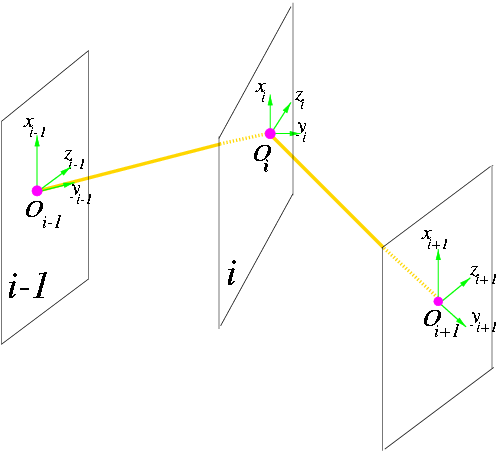
\includegraphics[width=6cm]{../images/jointplanes} &
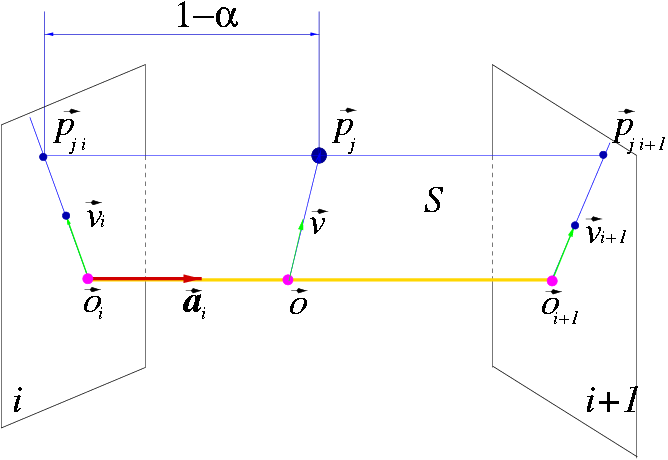
\includegraphics[width=6cm]{../images/point-to-line} \\
{\it (a)} & {\it (b)}
\end{tabular}
\caption[Joint planes and point-to-line mapping]{\label{fig:jointplanes} Joint plane mapping. (a) The joint planes bisect the angle of each joint. (b) Mapping points to a line, using the joint planes.}
\end{center}
\end{figure}

\subsection{\label{sec:chaindetail}High-Resolution Data Mapping}
After the control model has been mapped to the skeleton, the high-resolution detail layer is mapped onto the control layer. We map each point in the detail layer to a single triangle on the control layer, and parameterise the point in a coordinate system local to that triangle. As this is a mapping of a point to a surface, we need to use a different approach than that of the control mesh mapping. First of all, we decide which triangle a point will be mapped to, using the {\it normal volume} of the triangles in the control mesh, and then we parameterise that point in a system local to the triangle using a point-to-surface mapping.

\subsubsection{The Normal Volume}
The first step is to decide which control triangle a high-resolution point maps to. This is done using the normal volumes of the triangles in the control mesh. Every triangle $t_i$ has a volume of space associated with it called it's normal volume, $V^N(t_i)$. This is a volume which is triangular in cross-section and which extends above and below the triangle $t_i$, with it's edges following the directions of the normals of the vertices at the corners of the triangles. This is shown in figure \ref{fig:normalvolume}a. The normals at the the vertices are the average of the normals of the triangles incident on that vertex. We classify any point inside the normal volume of $t_i$ as belonging to that triangle. If a point is inside more than one normal volume, the triangle that is nearest to the point is used for mapping.

\begin{figure}
\begin{center}
\begin{tabular}{cc}
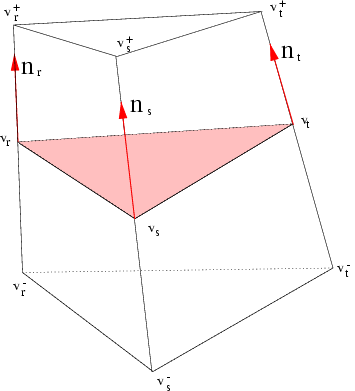
\includegraphics[height=5cm]{../images/normal_volume} &
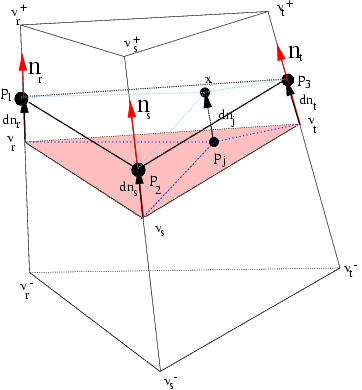
\includegraphics[height=5cm]{../images/point-to-surface} \\
{\it (a)} & {\it (b)}
\end{tabular}
\caption[Normal volume and point-to-surface mapping]{\label{fig:normalvolume} Normal volume mapping. (a) The normal volume of a single triangle. (b) A point is mapped onto a single triangle.}
\end{center}
\end{figure}

\subsubsection{Point-to-Surface Mapping}
Once we have decided which triangle a high-resolution point will map to, we need to do the actual mapping. Any point $\vec{p_j}$ on the triangle $t_i$ can be expressed in barycentric coordinates as $\vec{p_j} = \alpha\vec{v_r} + \beta\vec{v_s} + \gamma\vec{v_t}$, where $\vec{v}$ are the vertices at the corners of the triangle. Likewise, if we have normal information for each of the corners, we can express the normal $\vec{n_j}$ at the point $\vec{p_j}$ as $\vec{n_j} = \alpha\vec{n_r} + \beta\vec{n_s} + \gamma\vec{n_t}$, where $\vec{n}$ are the normals at the corners of the triangle. In both cases, $\alpha + \beta + \gamma = 1$ for any point inside the triangle, so $\gamma = 1 - \alpha - \beta$.

Using these two formulations, we can express any point $\vec{x}$ inside the normal volume of the triangle as:

\begin{eqnarray} \label{eqn:point}
\vec{x} & = & \vec{p_j} + d \vec{n_j}\nonumber \\
        & = & \alpha \vec{v_r} + \beta \vec{v_s} + \gamma\vec{v_t} + d( \alpha \vec{n_r} + \beta \vec{n_s} + \gamma\vec{n_t}  )\nonumber \\
        & = &  \alpha ( \vec{v_r}+ d\vec{n_r}) + \beta  ( \vec{v_s}+ d\vec{n_s}) + \gamma ( \vec{v_t}+ d\vec{n_t})
\end{eqnarray}

where $d$ is the distance along the normal $\vec{n_j}$ of the point $\vec{x}$ from the point $\vec{p_j}$. We can solve this equation for the three unknown coefficients, $\alpha$, $\beta$ and $d$. As the point $\vec{x}$, triangle vertices $(\vec{v_r},\vec{v_s},\vec{v_t})$ and normals $(\vec{n_r},\vec{n_s},\vec{n_t})$ are known three-dimensional vectors, we have three equations in three unknown variables. However, the variables are non-linearly related and therefore can not be solved for directly. A two step algorithm is used to solve this problem.

Firstly, $d$ is defined based on the fact that $\vec{x}$ is on the plane formed by $\vec{p_1} = (\vec{v_r}+d\vec{n_r})$, $\vec{p_s} = (\vec{v_2}+d\vec{n_s})$ and $\vec{p_3} = (\vec{v_t}+d\vec{n_t})$. The plane equation can be written as:

\begin{equation} \label{eqn:plane}
\vec{n}\cdot\vec{x} = \vec{n}\cdot\vec{p_1} = \vec{n}\cdot\vec{p_2} = \vec{n}\cdot\vec{p_3}
\end{equation}

where $\vec{n} = (\vec{p_2}-\vec{p_1}) \times (\vec{p_3}-\vec{p_1})$, the normal to the plane. This formulation is used to solve for $d$. Figure \ref{fig:normalvolume}b illustrates the plane through the point $\vec{x}$ defined by equation \ref{eqn:plane}. The plane is defined by the three points $(\vec{p_1}, \vec{p_2}, \vec{p_3})$ which are displacements by a distance $d$ along the vertex normals. It should be noted that each value of $d$ defines a unique plane. The union of these planes is a continuous volume which encloses all points in 3-space. Having obtained a solution for the variable $d$, the coefficients $\alpha$ and $\beta$ can be evaluated from equation \ref{eqn:point}. Figure \ref{fig:detailmapping} shows the results of the mapping of a detail layer to a control mesh. The triangles on the model shown in (c) are coloured according to the triangle that their vertices are mapped to. Triangles with vertices that map to more than one control mesh triangle are shown as white.

\begin{figure}
\begin{center}
\begin{tabular}{ccc}
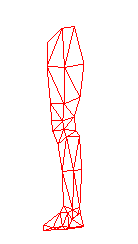
\includegraphics[height=6cm]{../images/lowres_leg} &
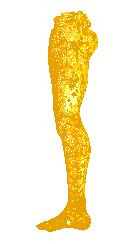
\includegraphics[height=5.75cm]{../images/dense_leg_1} &
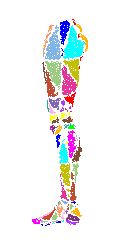
\includegraphics[height=6cm]{../images/leg_mapping} \\
{\it (a)} & {\it (b)} & {\it (c)}
\end{tabular}
\caption[Detail layer mapping]{\label{fig:detailmapping} Detail Layer Mapping. (a) Control mesh. (b) Detail Layer. (c) Mapping of detail layer points to control mesh triangles.}
\end{center}
\end{figure}

\section{\label{sec:chainanimation}Layered Animation}
As both the control layer and detail layer are now defined in terms of the local coordinate systems of part of the layer below, if we move the lowest layer (the skeleton), the higher layers will also move. The control mesh will change, as it is defined in the local systems of the skeleton segments, and the detail layer will change as it is defined in the local systems of the control mesh polygons. In this section, we will discuss how the layers are reconstructed from their mappings, and hence how animation of these layers is performed.

\subsection{\label{sec:chaincontrolanim}Control Layer}
As the skeleton layer is animated, the joints will change position, both globally and relative to one another. Therefore, the joint planes will also change. As our parameterisation of the space between the planes is based on the joint planes, the space between them is deformed as they move. This deforms the positions of the control mesh vertices which occupy that space. The method for calculating the new vertex positions is simple and efficient. Firstly, the joint planes are recalculated, either by using the new joint positions and calculating from scratch, or by rotating old joint planes by the appropriate amount (i.e. half of the joint's rotation).

We then use the stored normal for the point, $\vec{n_j}$, to calculate a vector on the upper plane and on the lower plane. The vector from the $\alpha$ point to the new vertex position, $\vec{p_{newj}}$ will be a linear interpolation of these two vectors based on $\alpha$. The upper and lower vector are calculated as the cross product of the stored normal with the upper and lower y axes.

\begin{eqnarray} \label{eqn:normals}
\vec{normal_i} & = & \vec{y_i} \times \vec{n_j} \nonumber \\ 
\vec{normal_{i+1}} & = & \vec{y_{i+1}} \times \vec{n_j} \nonumber
\end{eqnarray}

We can calculate the new point using these two normals. We calculate the $\alpha$-point by linear interpolation of the two joint positions, and the $\alpha$-normal (the normal at the $\alpha$-point) by linear interpolation of the two normals calculated above. The $\alpha$-normal is then multiplied by the stored distance $d_j$, and the two added together. The result is a new control mesh vertex, deformed by the correct amount dependent on the movements of the upper and lower joints.

\begin{equation} \label{eqn:rebuild}
\vec{p_{newj}}  = (1-\alpha_j)\vec{o_i} + \alpha_j\vec{o_{i+1}} + d_j((1-\alpha_j)\vec{normal_i} + \alpha_j\vec{normal_{i+1}})
\end{equation}

where $\vec{o_i}$ is the new upper joint position and $\vec{o_{i+1}}$ is the new lower joint position. As the only calculations performed for every point are linear interpolations, the reconstruction is highly efficient and can be performed in real time. A control model for a leg is shown at different stages of animation in figure \ref{fig:controlmesh}. Note how the shape of the segment deforms as the leg bends. The outer surface around the knee stretches, and the inner surface contracts. This gives a realistic yet efficient deformation. 

\begin{figure}
\begin{center}
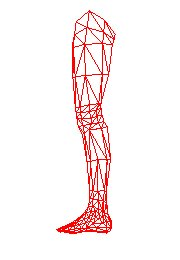
\includegraphics[width=3.18cm]{../images/low_leg_1}
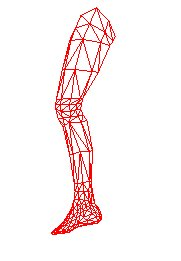
\includegraphics[width=3.18cm]{../images/low_leg_2}
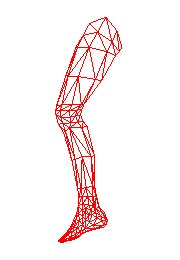
\includegraphics[width=3.18cm]{../images/low_leg_3}
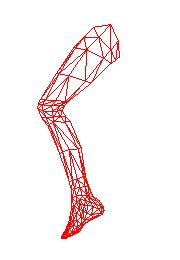
\includegraphics[width=3.18cm]{../images/low_leg_4}
\caption[Control Mesh Animation]{\label{fig:controlmesh} Control Mesh Animation.}
\end{center}
\end{figure}

A limitation of this method is that it does not currently handle twisting of segments well. The segment will tend to collapse in the middle as joints rotate about the segment axis. A better method of rebuilding the point is required to stop this problem, possibly involving interpolation of the rotation along the segment length. Also, the method as outlined above has a problem that under large joint rotations, the area around the joint will get noticeably thinner. A partial solution to this is obtained by adding a scaling factor to the magnitude of the joint plane vectors based on the joint angle, but this still will not deal correctly with very large rotations. A combination method of scaling and smoothing around the joint is required to deal with this problem. Both of these are important targets for future work on the deformation method.

\subsection{\label{sec:chaindetailanim}Detail Layer}
The point-to-surface mapping presented in section \ref{sec:chaindetail} can be used to map all vertices in a high-resolution mesh onto a low-resolution animation control model. This gives a high-detail object representation which can be animated efficiently using the control model. The problem then is to achieve a seamless smooth animation of the high-resolution model based on displacement of the control model.

If the low-resolution model geometry is modified such that vertices of triangle $t_j$ are changed to new positions $(\vec{v_{newr}}, \vec{v_{news}}, \vec{v_{newt}})$ and vertex normals are modified to $(\vec{n_{newr}}, \vec{n_{news}}, \vec{n_{newt}})$, then using equation \ref{eqn:point} we can evaluate for each original point $\vec{p_i}$ the position of a corresponding deformed point, $\vec{p_{newi}}$, on the high-resolution model as:

\begin{equation} \label{eqn:rebuilddetail}
\vec{p_{newi}} = \alpha_i(\vec{v_{newr}} + d \vec{n_{newr}}) + \beta_i(\vec{v_{news}} + d \vec{n_{news}}) + \gamma_i(\vec{v_{newt}} + d \vec{n_{newt}})
\end{equation}

As the new vertex position $\vec{p_{newi}}$ is only dependent on the triangle vertex positions and normals of the underlying low-resolution model, the high resolution model will deform efficiently and seamlessly as the low-resolution structure is manipulated.

Figure \ref{fig:detaillayer} shows animation of high-resolution captured data models. The dense leg model has 5102 vertices and 10200 triangles and the control model used (see figure \ref{fig:controlmesh}) only has 210 vertices and 416 triangles. These images show that that using our layered animation model, efficient and realistic animation of captured high-resolution data can be achieved. Future work on layered animation will explore alternative methods of generating the detail layer to give a more realistic real-time model. Possibilities for future expansion of this method are discussed in section \ref{sec:futuredetail}.

\begin{figure}
\begin{center}
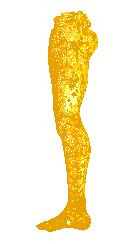
\includegraphics[width=3.18cm]{../images/dense_leg_1}
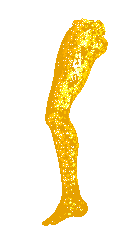
\includegraphics[width=3.18cm]{../images/dense_leg_2}
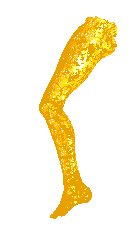
\includegraphics[width=3.18cm]{../images/dense_leg_3}
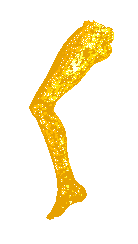
\includegraphics[width=3.18cm]{../images/dense_leg_4}
\caption[Detail Layer Animation]{\label{fig:detaillayer} Detail Layer Animation.}
\end{center}
\end{figure}

Figure \ref{fig:dino} shows an animation of a textured dinosaur model. A skeleton structure is fitted inside the tail, and a simple box model used as a control mesh. The image sequence shows reconstruction of the tail for different skeleton positions.

\begin{figure}
\begin{center}
\begin{tabular}{ccc}
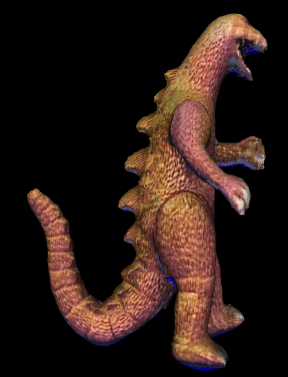
\includegraphics[width=4.3cm]{../images/dino1} & 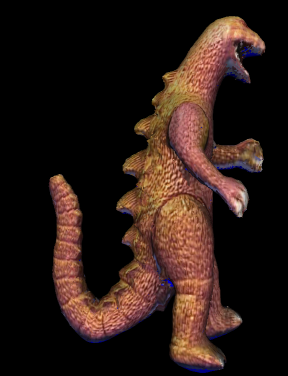
\includegraphics[width=4.3cm]{../images/dino2} & 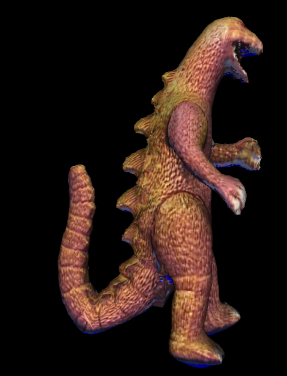
\includegraphics[width=4.3cm]{../images/dino3} \\
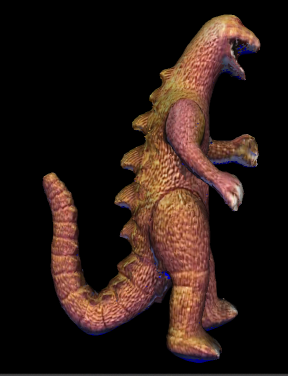
\includegraphics[width=4.3cm]{../images/dino4} & 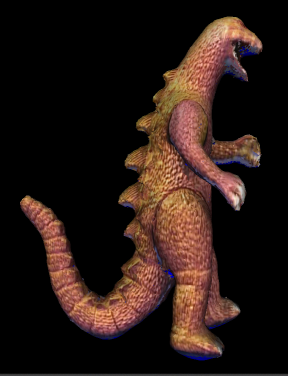
\includegraphics[width=4.3cm]{../images/dino5} & 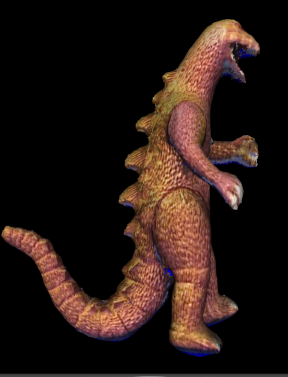
\includegraphics[width=4.3cm]{../images/dino6} \\
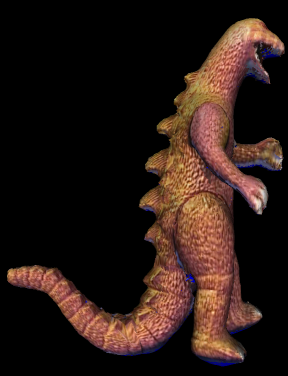
\includegraphics[width=4.3cm]{../images/dino7} & 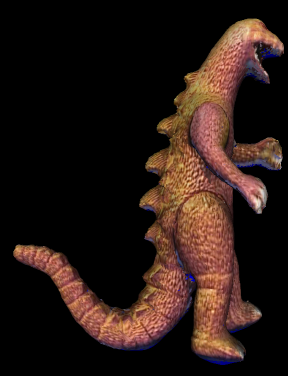
\includegraphics[width=4.3cm]{../images/dino8} & 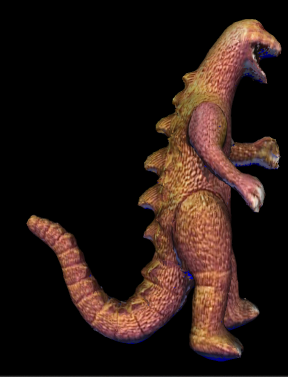
\includegraphics[width=4.3cm]{../images/dino9} \\
\end{tabular}
\end{center}
\caption[Dinosaur Animation]{\label{fig:dino}Dinosaur Animation. The dinosaurs tail is attached to a control mesh and skeleton, which is animated.}
\end{figure}

%%%%%%%%%%%%%%%%%%%%%%%%%%%%%%%%%%%%%%%%%%%%%%%%%%%%%%%%%%%%%%%%%%%%%%%%%%%%%%%%%%%%%%%%%%%%%%%%%%%%%%%%%%%%%%%%%%%%
\chapter{\label{ch:vrmlhumans}Seamless VRML Humans}
A large proportion of my work this year has been on the implementation of seamless deformable human models in VRML. The method used for this is basically the same as that for animation of the control layer in our layered models. There are a number of reasons why this work has been carried out.  

The first is that the quality of an animation method is entirely subjective, and cannot be calculated or visualised without seeing it in action. During the design of our animation process, implementation in VRML offered a quick method for viewing the results of our method without having to implement a complete 3D graphics system, as the models generated are viewed in a third-party browser. This is a major advantage, as it gives us the opportunity to implement the animation methods directly, without complex user interface design. Once we know that the animations we are creating are effective, we can continue with the earlier stages of the animation chain. 

Secondly, the seamless models also apply to work on another project with which I am not directly involved. This is the Virtual People project, which is carried out in conjunction with 3D Scanners, and involves creating models of people from a set of images. This project has recently been commercialised by 3D Scanners under a new company, AvatarMe. The seamless models developed here have been adopted by this new company as a way of representing their models in VRML. This is discussed further in section \ref{sec:vrmlavatarme}.

Finally, animation of rigid body segments, which is all that is currently possible in VRML, is not suitable for realistic objects. Seamless models have a much higher visual quality, and offer advantages such as surface and texture continuity. The layered model approach should be able to create realistic models for VR applications as well as for high-quality rendering, so some scheme for seamless animation in VRML is necessary.

We will now discuss the implementation of the control layer animation method in VRML. The implementation builds upon a previous standard for human body modeling, H-Anim \cite{HANIM99}. This is explained in the first section, followed by the work done to improve and extend this specification.

\section{\label{sec:vrmlhanim}H-Anim Compliant Humans}
The H-Anim 1.1 specification \cite{HANIM99} defines a standard representation for humanoid figures in VRML97 \cite{VRML97}. This standard defines a new set of VRML nodes used for representation of humanoid figures. These new nodes are implemented using the PROTO mechanism, defining new nodes in terms of combinations of old nodes. Because of this implementation method, the new nodes are subject to the same rules and restrictions as built-in VRML nodes.

At the top level, the humanoid is defined in a {\bf Humanoid} node. This in turn, contains a hierarchy of {\bf Joint} nodes, which make up the skeleton of the body. All joints are children of a higher-level joint, with the exception of the top-level joint, the {\bf HumanoidRoot} joint. This is a child of the Humanoid node itself. As all the joints are arranged in a hierarchy, rotating one joint will rotate all of its children in the same way. In this way, transformations propagate down the hierarchy. Joints are only allowed to rotate, not translate, meaning that distances between joints cannot change, and the skeleton retains the same basic shape and topology as it is moved. The joints contain a centre of rotation for the joint, as well as motion limit information.

The joints define the articulation structure, but not the shape of the body. This is done using {\bf Segment} nodes. Each joint has a child segment, corresponding to the part of the body attached below that joint. For instance, if we consider the {\it l\_shoulder} joint, it will have a child segment named {\it l\_upperarm}. The segments contain geometry information for that section of the body, so the {\it l\_upperarm} will typically contain an IndexedFaceSet node containing an arbitrary 3D model for the upper arm. However, the addition of seamless models has always been an aim of the H-Anim specification process, and to this end an extra field is included in the segment node that can contain a set of coordinates for part of such a model.

The segment node can also contain {\bf Site} nodes as children. These are used to store positions for feature points on the body, such as end effectors and attachment points for clothing and accessories. If we consider a segment representing the left hand, {\it l\_hand}, it will contain a site for use as an end effector, named {\it l\_hand\_tip}.

\section{\label{sec:vrmlextendinghanim}Extending H-Anim for Seamless Models}
Due to the limitations of VRML97, in particular the lack of support for non-linear transformations, H-Anim cannot support seamless models in pure VRML. However, we can use the {\bf Script} node of VRML97 to provide extra functionality not provided in the language, by programming it in Java or ECMAScript (commonly known as javascript). First, however, we need to define the VRML structure which will represent the seamless character. We will use H-Anim as a basis, as it is a standard format and a lot of our work is already done for use, such as the specification of the articulation structure. However, we need to add a number of new elements to H-Anim.

Our seamless models will take a different form than those described by Babski. His models consist of separate geometry for each segment, with the end of the segments held together to ensure a seamless appearance. We will take a different approach, and build a model that is truly a single surface. We start with a model which is a single surface, and separate the geometric properties of the model from it's topological and other properties. The vertices which define the position of the skin are split from the model and each one is assigned to a single segment according to it's position, during the modeling process. The rest of the model information, including connections between the vertices and any texture or colour information, is kept together in a single model. If we then move the skeleton, deforming the positions of the vertices in the segments, and fuse the vertices together in the same order in which they were created, we can place the new vertex positions back into the rest of the model, recreating the complete model. In this way, the surface topology and texture remain unchanged and only the vertex positions change, giving a seamless deformation of the model.

Each vertex of the model can be attached to a single body segment. We need to store these vertices somewhere, along with information about which segment a vertex is attached to. The H-Anim segment node contains a coordinate field, which has always been intended for use with seamless models. We will stay within the original intentions of the H-Anim group by using this field of a segment to store the vertices that belong to that segment.

We also need to create a placeholder object somewhere inside the Humanoid node which will store the remaining model information, and which will receive the coordinates of the deformed model to give a complete model. We define a new field in the Humanoid node, the {\it meshBody} field. This implemented as the child of a Group node which is itself a child of the Humanoid. This implementation puts the body into the transformation hierarchy at the same level as the very top of the articulation structure. When the body is moved as a whole in the world, the transformation is applied to the Humanoid node, and so will affect the deformable body model. However, is a transformation is applied to any part of the joint structure, the deformable body will not be directly affected. This is desirable, however, as these transformations correspond to changes in the body shape and as such require a recalculation, not transformation, of the deformable body. The extended Humanoid node is shown in figure \ref{fig:humanoidproto}.

\begin{figure}[t]
\scriptsize
\begin{verbatim}
PROTO Humanoid [
 exposedField SFString   name             ""
 exposedField MFString   info             []
 exposedField SFString   version          "1.1"
 exposedField MFNode     joints           []
 exposedField MFNode     segments         []
 exposedField MFNode     sites            []
 exposedField MFNode     viewpoints       []
 exposedField MFNode     humanoidBody     []
 exposedField SFNode     meshBody         NULL
 exposedField SFVec3f    center           0 0 0
 exposedField SFRotation rotation         0 0 1 0
 exposedField SFVec3f    scale            1 1 1
 exposedField SFRotation scaleOrientation 0 0 1 0
 exposedField SFVec3f    translation      0 0 0
]
{
  Transform {
    center IS center
    rotation IS rotation
    scale IS scale
    scaleOrientation IS scaleOrientation
    translation IS translation
    children [
      Group {
        children IS viewpoints
      }
      Group {
        children IS humanoidBody
      }
      Group {
        children IS meshBody
      }
    ]
  }
}
\end{verbatim}
\caption{\label{fig:humanoidproto} The extended Humanoid prototype}
\end{figure}

The new field will contain the body of our deformable model, which will be represented as an IndexedFaceSet node. This is a node that can contain an arbitrary mesh, along with colour, texture and normal information. We could just include an IndexedFaceSet node inside the meshBody field, but then we would have to find somewhere to put the deformation Script node as well. Instead, we can encapsulate both the body placeholder and the deformation engine in one node. Therefore, we define the new {\bf MeshBody} node, which will only be used inside the meshBody field of the Humanoid. This node is basically a fusion of the body placeholder and the deformation engine, an IndexedFaceSet and a Script. It has all of the fields of a normal IndexedFaceSet, with the exception of the {\it coord} field, which will be supplied by the deformation engine. The node also has the fields of a Script node, along with a series of eventIns, which will receive rotation and translation events passed on from the joint hierarchy. There is one eventIn for the rotation value of each joint, along with one for translation of the root joint. There is also a field called {\it humanoid}, which should contain a reference to the main Humanoid node. This is to allow the script to easily access members of this node, such as the joints and segments of the body. Note that the node also contains the {\it url} field for loading an arbitrary script, allowing the user to specify any deformation engine that works within this framework.

The internal structure of this node is basically just an IndexedFaceSet and a Script, and is very simple. The only special part is that the Script has a field that is not present in the MeshBody, the {\it bodyCoords} field. This is a reference to the coordinate part of the IndexedFaceSet, and allows the script to write values directly into this field, modifying the geometry of the body model. The MeshBody node prototype is shown in figure \ref{fig:meshbodyproto}.

\begin{figure}
\scriptsize
\begin{verbatim}
PROTO MeshBody [
 exposedField SFString   name             ""
 exposedField MFString   info             []
 exposedField SFNode     appearance       NULL
 exposedField SFNode     color            NULL
 exposedField SFNode     normal           NULL
 exposedField SFNode     texCoord         NULL     
 field        SFBool     ccw              TRUE
 field        MFInt32    colorIndex       []
 field        SFBool     colorPerVertex	  TRUE
 field        SFBool     convex           TRUE
 field        MFInt32    coordIndex       []
 field        SFFloat    creaseAngle      0
 field        MFInt32    normalIndex      []
 field        SFBool     normalPerVertex  TRUE
 field        SFBool     solid            TRUE
 field        MFInt32    texCoordIndex    []
 field        SFBool     mustEvaluate     FALSE
 field        SFNode     humanoid         NULL
 field        MFString   url              []
 eventIn      SFVec3f    HumanoidRoot_translation_changed
 eventIn      SFRotation HumanoidRoot_rotation_changed
 eventIn      SFRotation l_hip_rotation_changed
 eventIn      SFRotation l_knee_rotation_changed
 eventIn      SFRotation l_ankle_rotation_changed
 eventIn      SFRotation l_midtarsal_rotation_changed
 ...likewise for each joint...
]
{
  Group {
    children [
      Shape {
        appearance IS appearance
        geometry IndexedFaceSet {
          color IS color
          normal IS normal
          texCoord IS texCoord
          ccw IS ccw
          colorIndex IS colorIndex
          colorPerVertex IS colorPerVertex
          convex IS convex
          coordIndex IS coordIndex
          coord DEF BODYCOORDS Coordinate {}
          creaseAngle IS creaseAngle
          normalIndex IS normalIndex
          normalPerVertex IS normalPerVertex
          solid IS solid
          texCoordIndex IS texCoordIndex
        }
      }
      DEF SEAMLESSBODY Script {
        url IS url
        directOutput TRUE
        mustEvaluate IS mustEvaluate
        field SFNode humanoid IS humanoid
        field SFNode bodyCoords USE BODYCOORDS
        eventIn SFVec3f    translation  IS  HumanoidRoot_translation_changed
        eventIn SFRotation HumanoidRoot IS  HumanoidRoot_rotation_changed
        eventIn SFRotation l_hip        IS  l_hip_rotation_changed
        eventIn SFRotation l_knee       IS  l_knee_rotation_changed
        eventIn SFRotation l_ankle      IS  l_ankle_rotation_changed
        eventIn SFRotation l_midtarsal  IS  l_midtarsal_rotation_changed
        ...likewise for each joint...
      }
    ]
  }
}
\end{verbatim}
\caption{\label{fig:meshbodyproto} The MeshBody prototype}
\end{figure}

The topological and other data from our model is stored in the MeshBody node, in the same format as it would be generated by a modeling package. The vertices are distributed throughout the joint hierarchy, with their associated segments, and are deformed and fused by the deformation engine.

At this level of specification of the system, all that the deformation engine needs to do is read the rotations from it's eventIns, read the set of original coordinates from the segments, and output some set of new coordinates into it's bodyCoords field every now and again. As far as H-Anim extension is concerned, the deformation engine can be treated as a `black box' which is applied to the data. This allows the interface to be specified for seamless models, and work can be done on the internals of the deformation engine separately.

\section{\label{sec:vrmlmodeling}Modeling Seamless Humans}
The basic function of the deformation engine is to fuse the sets of vertices from the separate segments into one mesh. In order to do this, it needs to know what the order of the original vertices was. We perform this ordering during the modeling process, and assume this format inside the deformation engine. In the complete list of vertices for the model, the set of vertices for a segment must be contiguous, i.e. all the vertices for a segment must be ordered so that they are together. This also requires that the topology and texture information is ordered in the same way. This makes the vertices easier to fuse at the end of the deformation process. We output all of the vertices from one segment, followed by all of the vertices from the next, and so on. As long as we deal with the segments in the correct order, we will have the same ordering of vertices after deformation and fusion as in the original model. The order of the segments is not important as far as the modeler is concerned. The segments are entered in the correct vertex order into the {\it segments} field of the Humanoid, which contains references to Segment nodes. The deformation engine can extract this ordering of segments and fuse the vertices in the correct order.

Currently the only way to generate a model in this format is by using the AvatarConvertor software developed at Surrey (described in section \ref{sec:vrmlavatarconvertor}) to convert an AvatarMe avatar into a seamless H-Anim model. It is expected that this model segmenting requirement will be removed in a future revision of the seamless model specification (see section \ref{sec:futureseamless}), which will greatly ease the process of defining the model.

\section{\label{sec:vrmldeformation}The Deformation Engine}
As mentioned above, extra functionality is necessary to perform the deformation of the set of vertices. We can provide this through a VRML Script, which can be written either in ECMAScript of Java. We have chosen to implement the deformation in Java, as it is more structured that javascript, and is more suited to large and complex programs. The function of the deformation engine is to take the vertices from the original model, and transform them by the rotations and translations that are received through the Script's eventIns.

A Script in VRML works in the following way. On startup, an initialisation function is called. Then, whenever an event is received, an event handler is called. After a number of events have been processed (normally once per frame), a function called eventsProcessed() is called.

The initialisation method of our script will load all of the necessary information from the articulation structure, such as joint positions and segment vertices. This avoids wasting time loading information from the scene graph every frame. The event handler of the script will read the rotation values that are received and update the internal joints structure with the new rotations. The eventsProcessed function then performs all of the calculations necessary for the deformation process, and outputs the new set of coordinates into the bodyCoords field.

We will now discuss the method of deformation that is performed each frame. The deformation method has been built up in stages. The first stage is a rigid animation method, where the vertices in a segment are not deformed, but are subjected to a rigid transformation. The next stage is a method in which the vertices of simple segments (those that connect only two joints) are deformed based on joint angles.

\subsection{\label{sec:vrmlrigid}Rigid Animation}
The main aim of this animation stage was to ensure that the structure defined above was correct and would work as expected. The basic methods used in this stage of animation are also necessary for more detailed deformation.

Each frame, we have to start from the top of the skeleton structure and recalculate new global positions for the joints. This is done by creating a homogeneous transformation matrix, and recursively traversing the tree applying and updating this matrix. We start with the root joint, where we construct a matrix that corresponds to the translation and rotation of this joint. This is then passed to the children of the joint. These joints transform their original centre by the matrix, to get their current centre in global coordinates. This is stored, and their own rotation is added. They then apply this rotation to their child joints. In this way, the entire joint structure is traversed and all new joint positions calculated. The amount of calculation per joint is not dependent on the depth of the joint structure, as the computational cost for evaluating the new joint position is the same at all points in the hierarchy. Each joint also applies the transformation to any child Sites that it may have. These are not used at this level of deformation, but will be used later for segment deformation.

For rigid animation, the joints apply the transformation matrix to their child segment as the tree is traversed. The Segments apply this transformation to their set of coordinates, multiplying each coordinate by the matrix. This give a new set of coordinates, which are stored. 

Once the entire tree has been traversed, the new coordinates are extracted from each segment in order and fused into a single list, which is placed in the coordinate field of the IndexedFaceSet inside the MeshBody. An example of a model using rigid segment animation is shown in figure \ref{fig:rigidsegments}. Around the joints, it can be seen that the surface is not changing shape. The mesh self-intersects under the larger joint movements. Also, stretching of the triangles that cross joints can be seen in these cases.

\begin{figure}
\begin{center}
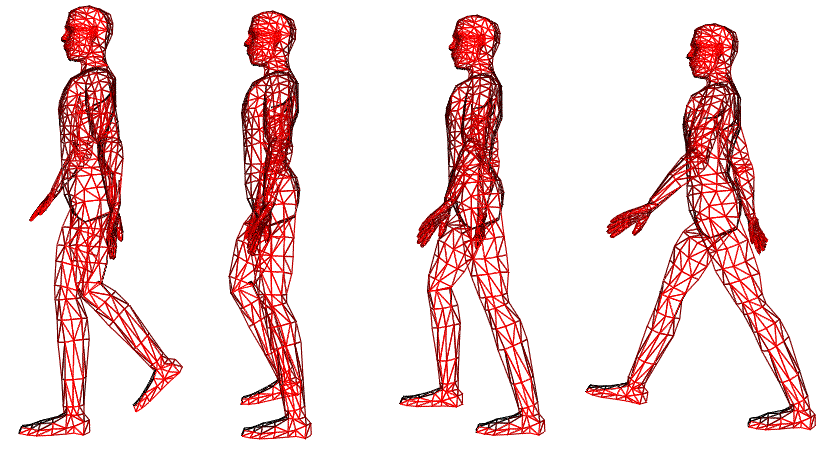
\includegraphics[width=14cm]{../images/rigidanimation}
\caption[Rigid Segment Animation]{\label{fig:rigidsegments} Rigid Segment Animation.}
\end{center}
\end{figure}

\subsection{\label{sec:vrmlsimple}Simple Segment Deformation}
The next level of realism in for the deformable models is to implement the control mesh animation method described in sections \ref{sec:chaincontrol} and \ref{sec:chaincontrolanim}. However, we do not need to do all of the work involved in this method, because we already know which vertices map to which segments. In the initialisation function, we map each vertex to the appropriate segment, storing a set of {\it deformation coordinates} in each segment. These are the $\alpha$ coordinate, the distance $d$ and the normal $n$. These are pre-calculated using the method described in section \ref{sec:chaincontrol}, and stored.

Each frame, the joints are moved, and the joint and site positions in the hierarchy are transformed as before. At this point, we can not yet deform the segments which join body parts, such as the pelvis and the torso. We can only transform the {\it simple segments}, which have only two bounding joints. The complex segments are rigidly transformed in the same way as before, using the transformation matrix.

Segments which are the child of a terminal joint (a joint with no child joint) do not have two bounding joints. This is overcome by treating some Sites as joints. If a joint is terminal, it will not have a child joint, but it should have a child Site, the {\it \_tip} sites mentioned above. In this case, the Site is considered to be a joint, and is used for mapping of terminal segments. Figure \ref{fig:skeleton} shows a skeleton structure of the sort that is used in this method. The skeleton is made up of joints, shown in blue, which are connected by segments. A simple segment has only two bounding joints, and a complex segment has more (shaded yellow segments). Each extremity of the model is terminated by a site (shown in green).

\begin{figure}
\begin{center}
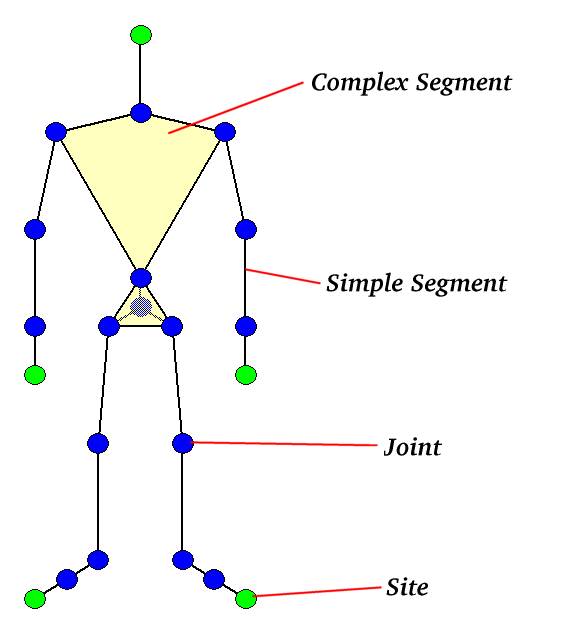
\includegraphics[height=7cm]{../images/skeleton}
\caption[Parts of the Skeleton Structure]{\label{fig:skeleton} Parts of the Skeleton Structure. Simple segments are those bounded by only two joints. Complex segments are bounded by more than two joints.}
\end{center}
\end{figure}

As the joint positions are updated, flags are set which can be used to test if the joints at either end of a segment have moved. If they have, the segment needs to be deformed. If not, the vertices of the segment can be rigidly transformed from the last frame, which is more efficient. Also, as the joint hierarchy is traversed, we rotate the joint planes. This is done by adding half of the rotation of a joint to the transformation matrix at that point, and then applying this to the vectors that define the joint plane. If a segment is to be deformed, it must be done after the entire hierarchy is updated and transformed, as the joint planes above and below must be updated before a segment can be calculated.

To deform a segment, we use the reconstruction method described in section \ref{sec:chaincontrolanim}. The cross products of the joint planes y-axes and the normal $n$ are calculated. These are then used in the linear interpolation equation \ref{eqn:rebuild} to recreate each deformed point. These are stored in the segment's working coordinate space, and fused together after every segment has been deformed, in the same way as for the rigid segments.

Figure \ref{fig:simplesegments} shows the same model as in figure \ref{fig:rigidsegments}, being deformed in this manner. The differences between rigid and deformable models can be seen around the knee joint as it moves. In the rigid model, the segments remain solid and do not change shape. In the deformable version, the vertices around the knee joint move to fill the gap created as the knee joint moves. Note, also, that there is no stretching across the joint, and that the back of the knee does not self-intersect.

\begin{figure}
\begin{center}
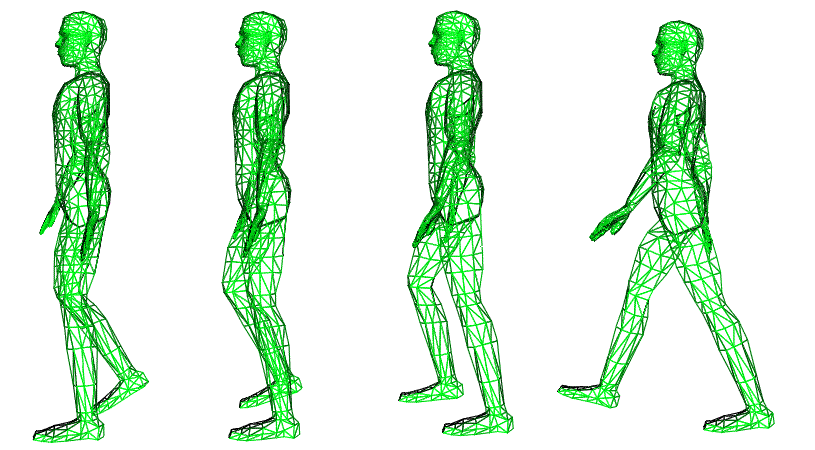
\includegraphics[width=14cm]{../images/simpleanimation}
\caption[Simple Segment Deformation]{\label{fig:simplesegments} Simple Segment Deformation.}
\end{center}
\end{figure}

\subsection{\label{sec:vrmlcomplex}Complex Segment Deformation}
Currently, neither the layered animation of the control mesh nor the VRML implementation of it can deal with complex segments. Complex segments are defined as those segments with three or more bounding joints (see figure \ref{fig:skeleton}). Currently, complex segments are simply transformed rigidly, without deformation. Ideally, the method for simple segment deformation could be extended to higher-dimensional volumes, allowing a simple bilinear or trilinear interpolation or joint planes to obtain new points. The deformation model itself should be an intuitive extension of the current simple segment method to higher dimensions. As a point at one end is affected a lot by it's nearby joint, and a little by the other, a vertex in a complex segment should have the same behaviour. The problem is how to deform the space based on more than two bounding planes.

The current method uses the $\alpha$ coordinate of a vertex as the most important factor in deformation. It is envisaged that a higher-dimensional deformation will use the same formulation of the reconstruction and mapping equations, albeit with more components. A 3-segment (a segment with three bounding planes) would have two ratio coordinates, $\alpha$ and $\beta$, while a 4-segment would also have a $\gamma$ coordinate. These are two-dimensional and three-dimensional barycentric coordinates respectively, and determine the ratio in which the normals at the joint planes are combined. This is a fairly straightforward extension of the deformation method to higher-dimensional spaces. 

There are only two types of complex segment found in a normal human body. The simpler of these are the 4-segments, as found in the pelvis (which contains the HumanoidRoot, the base of the spine, and the two legs), and the shoulders (top of spine, base of neck, and two arms). The more complex will only arise in models with complex articulation structures, but the method we choose should be able to handle them. These are 6-segments, which are found in the hands for joining the wrist and fingers in one joint. If we can find a method and parameterisation that extends well to 4-segments, hopefully it should extend in a similar way to 6-segments.

This problem is still open, however, and will be a major aspect of our future work in this project.

\section{\label{sec:vrmlavatarme}AvatarMe Integration}
The seamless human animation method described in this chapter can also be applied to another project in the CVSSP. The Virtual People project creates standard segmented H-Anim models from a set of four images of a person. This method has been commercialised by AvatarMe Ltd, and turned into a photo-booth style avatar creation machine. A person can stand inside, have their photograph taken from four angles, and then later download a model of themselves from the AvatarMe website. Originally, this system was going to use the segmented modeling approach developed at Surrey, but since our proposal for seamless VRML animation was introduced to them, they have altered their method to create seamless models instead.

\subsection{\label{sec:vrmlavatarconvertor}Avatar Conversion}
The software development kit created by AvatarMe for use with their AvatarBooth-generated models can be used to convert scanned models from the AvatarBooth into our seamless animation format. I have developed a windows application which allows easy conversion of the AMe models, and which is currently publicly available for download on the AvatarMe website. The software can create a textured, animated seamless model which can, in theory,  be viewed in any Java-capable VRML browser. Most of the Java classes required for seamless animation are installed as a plugin for Netscape or Internet Explorer, meaning that only a single Java class must be distributed with the model. The rest can be situated locally, reducing further the amount of data that must be transferred over the network. As these basic support classes are the same for every model, this is an ideal situation.

%%%%%%%%%%%%%%%%%%%%%%%%%%%%%%%%%%%%%%%%%%%%%%%%%%%%%%%%%%%%%%%%%%%%%%%%%%%%%%%%%%%%%%%%%%%%%%%%%%%%%%%%%%%%%%%%%%%%
\chapter{\label{ch:results}Results}
This chapter will show results of the seamless VRML animation technique described in the previous chapter. Obviously, most of the results are not quantifiable, the quality of an animation being subjective. Frame rate information for the models will be presented, which will show the increase in computation time for a seamless model, and also images of a number of seamless models generated from the AvatarMe software will be shown.

\section{\label{sec:resultcost}Computation Cost}
The extra calculation involved in generating the seamless models is measurable by considering the frame rate of a VRML browser displaying an animation of a model, for instance walking or running. A number of different resolutions of models have been generated, in order to show how the frame rate is affected by the number of points in a model. Not all of the models used to generate these results were actually converted into a seamless VRML character, due to lack of tools for point ordering. In a number of cases of rigid animation (marked in the table with a *), the entire model was attached to a single body segment in order to obtain a measurement for the frame rate with these models. This resulted in a model which still performed the same number of calculations, but did not move correctly. The results from these are still valid, however, as the computation time for such a model is the same as for a complete VRML character. This could not be done for the deformation method, as the results would not have been valid due to some of the calculations being optimised out, increasing the frame rate. The results are therefore somewhat incomplete, but are the best that could be obtained with current tools, and should still be sufficient show the general trend of the data. The results are shown in table \ref{tbl:framerates}.

\begin{table}[htbp]
\begin{center}
\begin{tabular}{|c|c||c|c|c|} \hline
\multicolumn{2}{|c||}{Model} & \multicolumn{3}{c|}{Frame Rate (frames per second)} \\ \hline
No. of Points & No. of Triangles & Segmented & Rigid & Deforming \\ \hline\hline
224 & 444 & 38.3 & 34.9 & 20.8 \\ \hline
1010*& 2014* & & 15.8 & \\ \hline
1290 & 2576 & & 14.7 & 10.1 \\ \hline
1734 & 2576 & & 16.6 & \\ \hline
11103 & 21422 & 7.1 & & \\ \hline
13202* & 26243* & & 2.4 & \\ \hline

\end{tabular}
\end{center}
\caption[Frame Rates for Seamless VRML models]{\label{tbl:framerates}Frame Rates for seamless VRML models.}
\end{table}

These measurements were made on a Pentium III 450MHz, with hardware OpenGL acceleration. The measurements were all taken while viewing the model in Cosmo Player running inside Netscape. It can be seen that the rigid segment deformation is quite inexpensive in terms of computation time, as the frame rate drop only slightly below that of a standard segmented model.

Currently the software is tested and works correctly in two VRML browsers, Cosmo Player ({\it http://www.cosmosoftware.com}) and Cortona ({\it http://www.parallelgraphics.com}), running inside either Internet Explorer or Netscape.

\section{\label{sec:resultappearance}Model Appearance}
A number of images are shown in figure \ref{fig:seamlessmodels}, which show seamless models converted from models captured by the AvatarMe AvatarBooth. These models all have the same basic topology, with the same number of vertices. The models have 1290 vertices and 2576 faces. Texture anomalies that can be seen on the models are artifacts of the capture process and model encoding, not the seamless animation, which provides perfect texture continuity. The same artifacts appear on completely static solid models of the figures.

\begin{figure}
\begin{center}
\begin{tabular}{ccc}
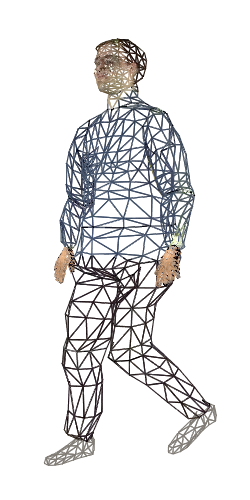
\includegraphics[height=6.5cm]{../images/boris_wireframe} & 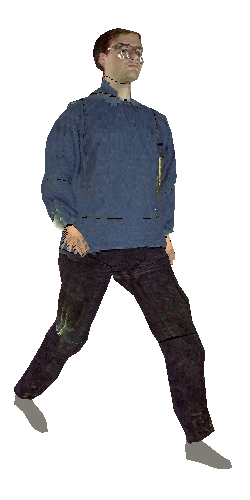
\includegraphics[height=6.5cm]{../images/boris_1} & 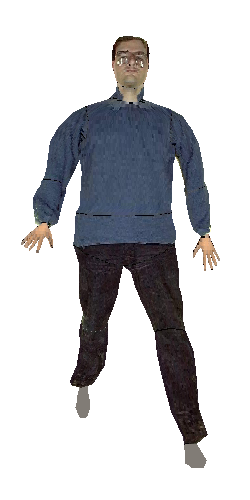
\includegraphics[height=6.5cm]{../images/boris_2} \\
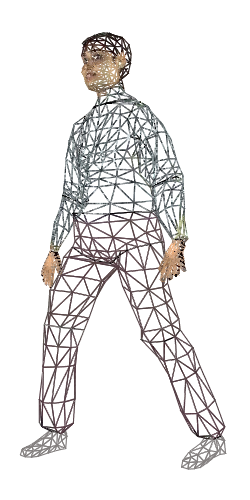
\includegraphics[height=6.5cm]{../images/rupal_wireframe} & \includegraphics[height=6.5cm]{../images/rupal_1} & \includegraphics[height=6.5cm]{../images/rupal_2} \\
\includegraphics[height=6.5cm]{../images/unknown_wireframe} & \includegraphics[height=6.5cm]{../images/unknown_1} & \includegraphics[height=6.5cm]{../images/unknown_2} \\
\end{tabular}
\end{center}
\caption[Seamless VRML models]{\label{fig:seamlessmodels}Seamless VRML models.}
\end{figure}

%%%%%%%%%%%%%%%%%%%%%%%%%%%%%%%%%%%%%%%%%%%%%%%%%%%%%%%%%%%%%%%%%%%%%%%%%%%%%%%%%%%%%%%%%%%%%%%%%%%%%%%%%%%%%%%%%%%%
\chapter{\label{ch:future}Future Plans}
So far, we have an initial method for creating layered models for animation. However, there is plenty of work to be done on the layered modeling chain in the future, as well as work on seamless VRML humans. The seamless humans are about to be put forward as a proposal for integration into H-Anim, and we will be participating in the process of creating the next version of the H-Anim specification. There are many things to be investigated in the layered model creation process, such as automatic creation of the control mesh, to allow reconstruction in cases where a generic model is not available. The layered animation method can also be expanded in many ways, such as allowing a more complex deformation of the control mesh. This also applies to the VRML human work. Finally, ways of reconstructing the detail layer for realtime animation will be investigated, to allow some representation of the detail layer to be added to the control mesh.

\section{\label{sec:futureseamless}Seamless VRML Models and H-Anim Integration}
The VRML Humanoid Animation Working Group have outlined a number of features that they would like to integrate into the next version of their H-Anim specification, version 1.2. Among these is a desire for a seamless model specification. As our method for seamless H-Anim has been adopted by AvatarMe, who have substantial influence in the H-Anim process, we believe that we will be playing a large role in the addition of seamless models to this specification over the next few months. We are currently about to propose the method outlined in this report to the group, along with some possible alterations.

These alterations include the removal of the vertex positions from the individual segments. The vertices will instead be stored in the MeshBody, along with the rest of the model definition. The segments will have numerical references to the vertices in the MeshBody, so that the vertices for a particular segment can still be found. This arrangement has three main advantages:

\begin{itemize}
\item The vertices of the model no longer have to be reordered for placing into the segments, as the numerical references stored in the segments can refer to any vertex in the complete list. This removes the only modeling constraint of our current method, making models easier to create.
\item Vertices can be attached to more than one segment, allowing future implementation of much more complex deformation schemes.
\item As the body is now stored as a complete model, if the deformation engine cannot be found, the model will still appear in the world. It will not animate, but it will at least be visible. This is obviously highly desirable. We would also like to make this rigid model animate without Java. This will requires some redesign of our method, but would be extremely useful.
\end{itemize}

This change of model format would require very little change in the code for our current deformation engine, and would confer all of the highly desirable advantages listed above. It is anticipated that our proposal will follow this improved version of our current method.

\section{\label{sec:futuremesh}Mesh Optimisation}
The current method of layered model building allows the user to use a pre-generated low-resolution model of the object as a control model. This can be either a professionally created model from a model library, or it can be a heavily decimated or remodeled version of the scan data. In either case, some manual intervention is required to create the control model. Also, the skeleton must be fitted to both the control and the detail models. Ideally, there would only be one fitting stage, in which the skeleton is fitted inside the detailed model. Then, a control mesh could be automatically generated from the detailed model. This would cut user intervention still further, and give the advantage that a pre-generated generic model is not required. This would be very useful in that case of unusual models, such as aliens or other common animated characters. Investigation is required into the possible approaches to automatic generation of the control model, but some possibilities include:

\begin{itemize}
\item Decimation of the detail model. This could be uncontrolled, or constrained on the basis of the skeleton positioning inside the body. However, it may be difficult to control how the control mesh is structured using normal decimation techniques. Possibly using the edge collapse method described by Hoppe \cite{Hoppe93}, the decimation of the detail layer down to the control layer could be controlled more precisely.
\item Retriangulation of the detail layer. The detail layer could be retriangulated into larger polygons, possibly after conversion back to an implicit surface. This, however, may be very computationally expensive.
\item Raycasting from the skeleton to the detail layer. Once the skeleton is added, the surface generation approach used by Shen \cite{Shen95} for skin creation from metaball models could be adapted to create a control mesh. At certain points on each segment, rays are cast orthogonally from segment to the skin surface. The intersection points are then joined to create a low-resolution, well-structured mesh.
\end{itemize}

Of these, I would suggest that the last is the most promising, as it aims to create a structured mesh (Shen's models are highly structured) which is based completely on the shapes of the skeleton and the detailed model.

\section{\label{sec:futureanimation}Realtime Animation}
There is a large amount of work that can be done to improve the animation of layered models. These include increasing the efficiency of the representation to allow more complex realtime animation, and increasing the power of the deformation model that is applied to the data to allow more complex methods of deformation. 

\subsection{\label{sec:futureparam}Alternative Parameterisations}
There are many different possible parameterisations for the point-to-line mapping of the control mesh. This is an important area to investigate, as alternative parameterisations may allow better storage efficiency and quicker surface reconstruction. One particular parameterisation has already been considered, which stores the $\alpha$ value of a point, along with a coordinate in a local plane, where the local plane is a combination of the two end planes. This particular parameterisation has only three components, as opposed to five for the current method. Reconstruction from these parameters could also be more efficient. Parameterisations for complex segments must be considered. Ideally, one style of parameterisation should be able to represent both the simple and complex segment mappings. The creation of a general mapping and animation method that applies for a segment with any number of bounding planes would be a valuable piece of work, and is an important part of our future research. The proposed 3-component parameterisation has the property of extending naturally to complex segments.


\subsection{\label{sec:futuredeformation}Extending the Deformation Model}
The formulation for reconstruction of the control mesh is very simple, as it is a linear combination of the two end values. This, however, gives a very simple deformation model, with a number of limitations. Work is required on extending this model, and adding extra functionality for dealing with twisting of segments and smooth rounding at joints. This can be done by replacing the $\alpha$ and $1-\alpha$ coefficients in the reconstruction equations with an arbitrary function, $f(\alpha)$, which can provide the extra functionality. The operation of this function is unknown currently, but work will be carried out researching possible formulations. 

\section{\label{sec:futuredetail}Surface Detail Representation}
The current method of detail layer reconstruction is efficient, and gives a realistic model. However, it is not fast enough to be usable in real time. Interaction with a detail-layer model would be beyond the capabilities of most current computing systems. However, a lot of information about the model is contained in the detail layer, so it is desirable to find a more efficient way to represent this information. Ideally, we should be able to develop a method that can use the detail layer of a model if computing power allows it, and if not, falls back on either a lower-resolution version of the detail layer, or another representation of it. Possibilities for investigation are:

\begin{itemize}
\item Transformation of detail layer into a texture or bump map, for simple mapping onto the control mesh. This would make the model appear more realistic during animation design.
\item Displacement mapping. Again, the detail layer could be converted into a displacement map which can be added to the control mesh to add extra realism. Techniques for animating displacement maps need to be investigated.
\item Mesh Subdivision. The control mesh could be refined, based on the detail layer. Individual triangles can be subdivided, following the surface of the detail layer. If this can be done dynamically, there is the possibility of implementing distance or gaze-controlled level of detail for the models.
\end{itemize}

Future research will investigate the combination of the last two points to generate a `subdivision displacement map'. This would give highly efficient image based representation of surface detail, together with multiple levels of detail for efficient rendering. This offers the possibility of efficient storage and transmission for Internet based applications of virtual humans.

%%%%%%%%%%%%%%%%%%%%%%%%%%%%%%%%%%%%%%%%%%%%%%%%%%%%%%%%%%%%%%%%%%%%%%%%%%%%%%%%%%%%%%%%%%%%%%%%%%%%%%%%%%%%%%%%%%%%
\chapter{\label{ch:conclusion}Conclusion}
This report has detailed work carried out during my first year in the CVSSP. We have covered the background to the computer modeling and character animation fields, and then discussed our novel method for building layered models that are suitable for animation.  We then showed an implementation of these models in VRML, which has the prospect of being built into a standard humanoid model representation. Future work in the field was also discussed, and will concentrate on improved animation of the layered models, including variable levels of detail for efficiency and realism.

In brief, the work I have been directly involved in that has been covered in this report includes:

\begin{itemize}
\item Defining the layered animation model.
\item Animation of control meshes in the layered animation model.
\item Implementation of control mesh animation in VRML.
\item Creation of a specification for definition of seamless human models in VRML.
\item Commercial application of these seamless models, through the conversion software for AvatarMe.
\end{itemize}

Future work will concentrate on the following areas:

\begin{itemize}
\item Automatic creation of the control mesh from the detail layer, or scanned data.
\item Better deformation methods for the control mesh, including complex segment deformation.
\item Animation of bump or displacement maps for surface detail representation in real time.
\item Integration of our seamless human proposal into H-Anim.
\end{itemize}

At present, it is expected that my thesis will concentrate on animation of the control mesh layer, with real time, variable level-of-detail animation of the detail layer, particularly when applied to seamless human models in VRML.


\bibliographystyle{abbrv}
\bibliography{../bib/papers,../bib/r.smith}

\end{document}
